\documentclass[12pt,a4paper]{book}
\usepackage[brazil]{babel}
\usepackage[utf8]{inputenc}
\usepackage{amsmath, amsthm, amssymb}
\usepackage{setspace}
\usepackage{xypic}
\usepackage{cite}
\usepackage{changepage}
\usepackage{mdframed}
\usepackage{mathrsfs}
\usepackage{multicol}
\usepackage{comment}
\usepackage[colorinlistoftodos,prependcaption,textsize=tiny]{todonotes}
\usepackage{lscape}
\usepackage[toc,title]{appendix}
\usepackage{tabularx} 
\usepackage{caption}
\usepackage{longtable}
\usepackage[osf,sc]{mathpazo}
\usepackage{hyperref}
\usepackage{imakeidx}
\makeindex

\makeindex[name=sage,title={Funções e Métodos \Sage}]


%% RASCUNHO
\usepackage{draftwatermark}
\SetWatermarkText{RASCUNHO}
\SetWatermarkScale{1}
\SetWatermarkAngle{60}

\usepackage{fancybox}

\usepackage{aurical}
\usepackage[T1]{fontenc}


\usepackage{hyperref}
\usepackage{xspace}
\newcommand{\Sage}{\emph{sagemath}\xspace}
\newcommand{\sage}{\emph{sagemath}\xspace}

\allowdisplaybreaks

\newcommand\todoin[2][]{\todo[inline, caption={TODO}, #1]{
\begin{minipage}{\textwidth-4pt}#2\end{minipage}}}

% gambiarra pra ajeitar as margens
\usepackage[dvips]{geometry}
\geometry{a4paper, left=1in, right=1in, top=1in, bottom=1in}

%%% 
\title{Teoria dos Números Básica com o \Sage}
\author{Vinicius Martins Teodosio Rocha}
\date{}
%%%

%alias
\newcommand{\ZZ}{\mathbb{Z}}
\newcommand{\RR}{\mathbb{R}}
\newcommand{\FF}{\mathbb{F}}
\newcommand{\CC}{\mathbb{C}}
\newcommand{\QQ}{\mathbb{Q}}
\newcommand{\NN}{\mathbb{N}}
\newcommand{\PP}{\mathbb{P}}

\newcommand{\cA}{{\cal A}}
\newcommand{\cO}{{\cal O}}
\newcommand{\cE}{{\mathscr E}}
\newcommand{\cX}{{\cal X}}
\newcommand{\cT}{{\cal T}}
\newcommand{\cS}{{\cal S}}
\newcommand{\cK}{{\cal K}}
\newcommand{\cV}{{\cal V}}
\newcommand{\cW}{{\cal W}}


\newcommand{\ts}{\textsuperscript}

\newcommand{\supp}{{\rm Supp}}
\newcommand{\tsb}{\textsubscript}

\newcommand{\Pic}{\operatorname{Pic}}
\newcommand{\Spec}{\operatorname{Spec}}
\newcommand{\Proj}{\operatorname{Proj}}
\newcommand{\Div}{\operatorname{Div}}
\newcommand{\Tr}{\operatorname{Tr}}
\newcommand{\Gal}{\operatorname{Gal}}
\newcommand{\rk}{\operatorname{rk}}
\newcommand{\tors}{\operatorname{tors}}
\newcommand{\Sec}{\operatorname{Sec}}
\newcommand{\Id}{\operatorname{Id}}
\newcommand{\Het}{H_{\text{ét}}}
\newcommand{\rank}{\operatorname{rank}}
\newcommand{\Frob}{\operatorname{Frob}}
\newcommand{\res}{\operatorname{res}}
\newcommand{\Diff}{\operatorname{Diff}}
\newcommand{\NS}{\operatorname{NS}}
\newcommand{\Km}{\operatorname{Km}}
\newcommand{\Hom}{\operatorname{Hom}}
\newcommand{\End}{\operatorname{End}}
\newcommand{\MW}{\operatorname{MW}}
\newcommand{\mdc}{\operatorname{mdc}}
\newcommand{\sgn}{\operatorname{sgn}}
\newcommand{\legendre}[2]{\left(\frac{#1}{#2}\right)}


% especiais


%alias fim

\pagestyle{headings}
\newtheorem{theorem}{Teorema}[chapter] %chapter
\newtheorem{conjecture}[theorem]{Conjecture}
\newtheorem{corollary}[theorem]{Corollary}
\newtheorem{proposition}[theorem]{Proposição}
\newtheorem{lemma}[theorem]{Lema}
\theoremstyle{definition}
\newtheorem{definition}{Definição}
\newtheorem{exercise}{Exercício}[chapter] 
\newtheorem{example}{Exemplo}[chapter] 

\usepackage{listings}


\newcommand{\ils}[1]{\texttt{\color{black}{\colorbox{sageblue}{#1}}}}
\newcommand{\ilso}[1]{\texttt{\color{black}{\colorbox{lightgreen}{#1}}}}
\newcommand{\red}[1]{\color{red}#1\color{black}}
\newcommand{\blue}[1]{\color{blue}#1\color{black}}


% \onehalfspacing
% \doublespacing

\usepackage{tcolorbox}
\tcbuselibrary{skins}
\tcbuselibrary{breakable}
\tcbuselibrary{raster}
\tcbuselibrary{listings}
\definecolor{sageblue}{HTML}{8BBEB2}
\definecolor{lightgreen}{HTML}{E6F9AF}%{1B264F}
\definecolor{sageintext}{HTML}{0D0630}
\definecolor{sageouttext}{HTML}{0D0630} %{F5F3F5}
\tcbset{ sagestylein/.style={left=0pt, right=0pt, top=0ex, bottom=0ex, middle=0pt, toptitle=0pt, bottomtitle=0pt,
boxsep=4pt, listing only, fontupper=\small\ttfamily,
breakable, parbox=false, 
listing options={language=Python,breaklines=true ,breakatwhitespace=true, extendedchars=true, aboveskip=0pt, belowskip=0pt,numbers=left}} }
\tcbset{ sagestyleout/.style={left=0pt, right=0pt, top=0ex, bottom=0ex, middle=0pt, toptitle=0pt, bottomtitle=0pt,
boxsep=4pt, listing only, fontupper=\small\ttfamily,
breakable, parbox=false, 
listing options={language=Python,breaklines=true ,breakatwhitespace=true, extendedchars=true, aboveskip=0pt, belowskip=0pt}} }

\newtcblisting{sageinput}{sagestylein,  colback=sageblue, sharp corners, boxrule=0.5pt, toprule at break=-0.10pt, bottomrule at break=-0.3pt, 
coltext=sageintext}
\newtcblisting{sageoutput}{sagestyleout, colback=lightgreen, colframe=white, frame empty, before skip=0pt, after skip=5pt,coltext=sageouttext,}


\usepackage{showlabels}

\begin{document}
\maketitle
% \thispagestyle{empty}
%  \begin{tikzpicture}[remember picture,overlay]
%    \node at (current page) {
\includegraphics[width=\pdfpagewidth,height=\pdfpageheight]{capa/capa2.png}};
%  \end{tikzpicture}
\clearpage

\frontmatter
\tableofcontents

\chapter*{Prefácio}
\addcontentsline{toc}{chapter}{Prefácio}


O \sage é um poderoso software para a manipulação de objetos matemáticos.
É um software gratuito e de código aberto, sob a licensa GPL, construído
sobre diversos outros pacotes, também de código aberto, como o NumPy, 
SciPy, matplotlib, Maxima, GAP, R, etc.  Baseado na linguagem de programação
Python é uma ótima ferramenta para explorar conceitos matemáticos. 

Nesse texto usamos o \sage para explorar a área da matemática
conhecida como teoria dos números, ou aritmética. O \sage possui
uma enorme gama de recursos relacionados à teoria dos números
básica, além de dispor de métodos que auxiliam a construção de
ferramentas para nossas próprias investigações.

Sendo baseado em Python, o \sage consegue executar qualquer
comando ou script Python da forma esperada (a menos
de um conjunto de medida nula). 
Com o risco de exagerarmos no tom informal, tentamos evitar ao máximo
o uso conhecimentos prévios sobre a linguagem Python e sobre
algoritmos de uma forma geral. Evidentemente, alguns
conceitos e técnicas apresentados fazem uso de conhecimentos 
específicos de algoritmos, mas \textbf{não é necessário
saber programar} para seguir essas notas, basta estar disposto
a aprender.

Aproveitamos para destacar que existe uma 
enorme quantidade de recursos do \sage que não
abordaremos em detalhes, como o cálculo simbólico, a construção de gráficos 
integrado ao matplotlib, objetos da álgebra abstrata,
como grupos e aneis, combinatória, computação numérica...
Dessa forma, instigamos ao leitor que faça um passeio
pela documentação do \sage (\cite{sagedoc}) e descubra outras ferramentas
disponíveis que podem auxiliá-lo no seu dia a dia de estudante
ou professor, além da documentação dos recursos, também há diversos
tutoriais ou materiais sobre temas específicos e uma lista é mantida
com os livros e publicações sobre o \sage.
Recomendamos também o ótimo livro \cite{sagesbm},
única referência em português sobre o \sage de conhecimento
do autor. Em inglês há mais recursos, destacamos
\cite{zimmermann2018computational} (Versão em inglês, original
francês) e \cite{bard2015sage} (Versão em inglês, também
disponível em espanhol), ambos com versões gratuitas 
disponíveis nos sites dos autores e contendo ao menos
um capítulo sobre teoria dos números..



SEPARADOR

Ao escrever essas notas fizemos algumas escolhas sobre o estilo e o conteúdo
que necessitam justificativa.
Com o intuito de não tornar esse texto mais longo que deveria, optamos
por omitir algumas demonstrações e discussões
mais teóricas, indicando referências mais adequadas
(e decerto mais bem escritas) para o que for omitido. Dessa forma, essas notas 
não tem como objetivo substituir um texto mais formal de teoria dos números,
com todas as propriedades, teoremas e demonstrações.
A exceção  ocorre quando as demonstrações são, de alguma forma, construtivas.
Nesse caso procuramos fornecer um esboço da demonstração que
auxilie na construção de um código \sage.

Apesar do nosso objetivo principal ser a apresentação do \sage
como uma ferramenta pronta para o uso, também gostaríamos que
o leitor desenvolvesse um raciocínio lógico que o permita
transpor uma lista simples de procedimentos em linguagem matemática
para código \sage. Para tal iremos apresentar a construção de algumas
ferramentas básicas que já estão implementadas no sage, então, sim,
em alguns momentos estaremos \emph{reinventando a roda}, mas cremos
que esse é um passo importante para o entendimento dos 
algoritmos mais avançados que apresentaremos ao final do texto.

Para os que já são familiarizados com a linguagem Python, inserimos algumas
observações onde o \sage supostamente funciona de forma diferente do Python,
ou onde objetos ligeiramente diferentes são usados.
Para os que não são familiarizados com o \sage ou Python, optamos por
não inserir uma longa seção  inicial tratando de sintaxe,
lógica de programação, etc. Vamos direto ao ponto e espalhamos essas explicações
aqui e ali, na medida que se fazem necessárias. Para os leitores
mais sistemáticos, os três primeiros
capítulos do já citado \cite{sagesbm} fornecem uma introdução
completa ao \sage, sugerimos sua leitura antes de explorar
esse texto.

{\color{blue} Descrição capítulo a capítulo}

Inserimos em cada capítulo uma seção 
chamada \textbf{Explore!}, onde descrevemos
alguns tópicos adicionais
que acreditamos serem aplicações interessantes. Dentro
de cada tópico há alguns
exercícios mas, para alguns deles,  o instrutor pode desenvolver miniprojetos
estendendo o escopo abordado. No final de cada capítulo
há uma seção \textbf{Exercícios}, com problemas adicionais,
generalizações de resultados ou implementações alternativas
às mostradas no corpo do texto. Tais exercícios
não são, em geral, fundamentais para a
compreensão do assunto. Por outro lado, no corpo do texto
há determinados exercícios que julgamos essenciais
para o desenvolvimento da aprendizagem, alguns,
inclusive, podem não fazer muito sentido se ignorados e
deixados para depois.
Tentamos indicar
os exercícios mais trabalhosos ou que exigem um 
aprofundamento das técnicas com um sinal X, no entanto
nenhum requer assuntos não abordados, exceto 
menção explícita a alguma referência.


\mainmatter

\chapter*{Introdução}
\addcontentsline{toc}{chapter}{Introdução}

\section*{O \sage}

Apresentamos brevemente como utilizar o \sage e alguns conceitos
básicos.

Há diversas formas de se trabalhar com o \sage, e uma de suas vantagens
é que você nem precisa ter o \sage instalado em seu computador 
para usá-lo. Na prática, não há muitas razões para a maior parte
dos usuários instalar o \sage. 

De toda forma, se optar pela
instalação, siga as instruções em \url{https://www.sagemath.org/download.html}.
Após a instalação a forma mais direta de utilização é através
da linha de comando: abra uma linha de comando, digite \ils{sage}
e, voilá, você já está dentro do interpretador interativo \sage.
Tente digitar algum código

\begin{sageinput}
2+2
\end{sageinput}
\begin{sageoutput}
4
\end{sageoutput}

Usaremos o padrão acima nessas notas, o texto no quadro azul
é o código \sage e o texto no quadro verde é o resultado do código
acima. 
No interpretador \sage, qualquer código sage válido inserido
será executado e você verá o resultado na hora. Para 
códigos mais elaborados o mais usual é salvá-lo em um arquivo com a extensão
\ils{.sage} e executar o comando \ils{sage} na linha de comando
com o arquivo como argumento. No entanto, a interface mais amigável para o
\sage é fornecida pelo Jupyter, um projeto para o desenvolvimento de padrões
para computação interativa. Ao utilizar o \sage em um notebook Jupyter
você vai trabalhar em um página web local, através do seu navegador,
como na Figura \ref{fig:jupyter}.

\begin{figure}[h]
  \centering
  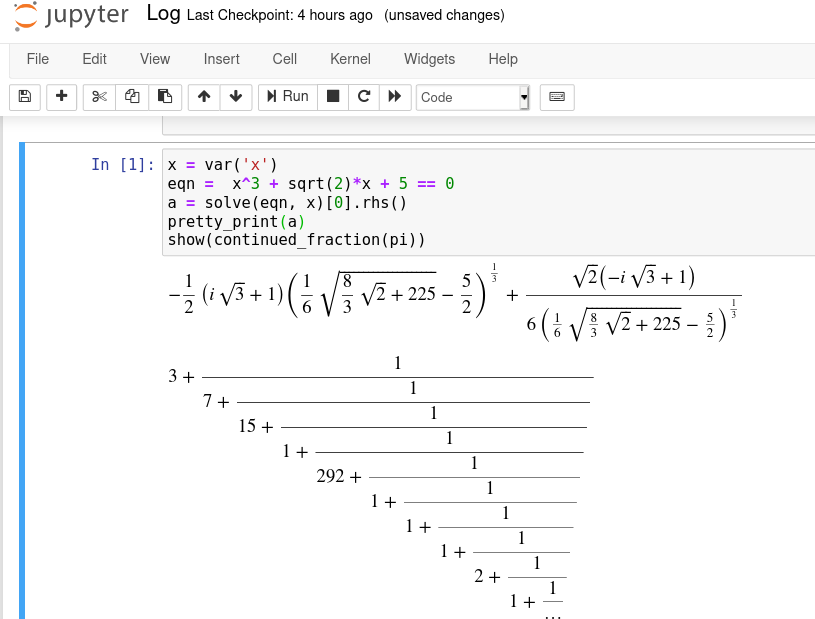
\includegraphics[scale=0.4]{imgs/jupyter.png}
  \caption{Tela do \emph{Jupyter}}
  \label{fig:jupyter}
\end{figure}

Par a maior parte das pessoas, no entanto, recomendamos
a utilização de alguma opção \emph{online} do \sage. Há duas
opções principais. A mais simples e direta de todas é utilizar
a célula de cálculo no site \emph{SageMathCell}, 
acessado em \url{https://sagecell.sagemath.org}. Nesse site
você verá um campo de texto onde pode inserir código \sage. Em
seguida basta clicar em \emph{Evaluate} para ver o resultado,
como na Figura \ref{fig:sagemathcell}.  Todos os códigos
utilizados nesse texto podem ser executados no
\emph{SageMathCell}. Vale destacar, no entanto, que ao fechar o site
todo o seu código será perdido, bem como o resultado. Dessa forma
se quiser salvar o seu trabalho, você pode copiar o código que digitou
no \emph{SageMathCell} e salvar em um arquivo de texto, podendo
voltar a trabalhar nele em outro momento.

\begin{figure}[ht]
  \centering
  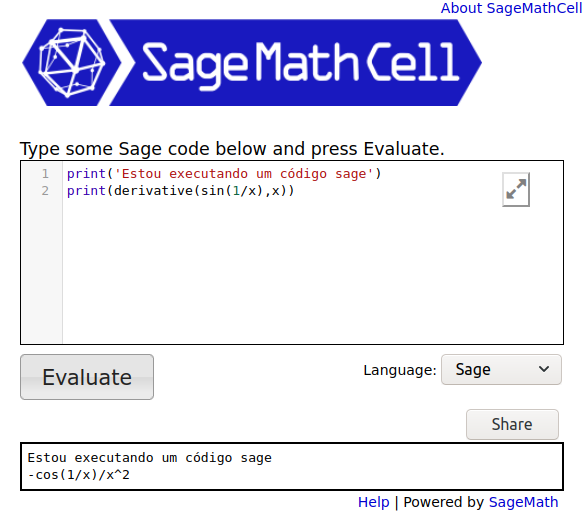
\includegraphics[scale=0.4]{imgs/sagemathcell.png}
  \caption{Tela do SageMathCell}
  \label{fig:sagemathcell}
\end{figure}

Outra opção, que evita o problema de perder os códigos, é usar
o \emph{CoCalc}, uma plataforma online permitindo o uso
de diversas ferramentas, incluindo o \sage. Apesar de existirem 
diversos planos pagos, fornecendo mais capacidade
de memória e processamento, há uma
versão gratuita que é o suficiente para grande parte
das aplicações. Ao criar uma conta no site do \emph{CoCalc}, 
você poderá criar arquivos e projetos de diversos tipos. 
Estaremos interessado em particular em \emph{worksheets \sage},
arquivos no formato \ils{.sagews}, que funcionam de forma parecida
com notebooks do Jupyter\footnote{também é possível usar o Jupyter
com o \sage dentro do Cocalc}. A grande vantagem é que os
seus arquivos ficarão salvos na sua conta, mesmo após o
fechamento do navegador, além disso você pode trabalhar
colaborativamente com outros colegas no mesmo arquivo.

\begin{figure}[h]
  \centering
  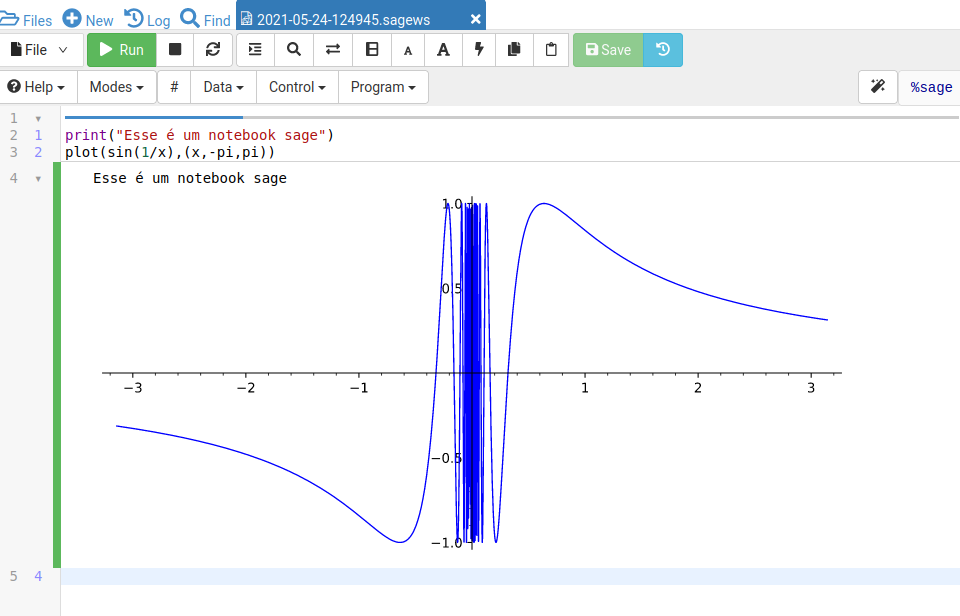
\includegraphics[scale=0.4]{imgs/cocalc.png}
  \caption{Tela do \emph{CoCalc}}
  \label{img:cocalc}
\end{figure}


O \emph{CoCalc} e o \emph{Jupyter} fornecem diversas outras
ferramentas, recomendamos que o leitor acesse os sites
dessas plataformas e descubra quais dessas ferramentas pode
achar útil. Como comentamos, para essas notas, o uso
do \emph{SageMathCell} será suficiente.


Vemos a seguir alguns conceitos básicos sobre o \sage. 


\paragraph{Conjuntos Numéricos} Os objetos mais básicos
que utilizaremos serão os números. Sabemos que o número
$12$, por exemplo, é um número inteiro, racional, real
e complexo. No \sage, no entanto, faz certa
diferença onde os números estão sendo considerados. Não
fará sentido, por exemplo, perguntar ao \sage 
a fatoração em primos de \ils{12.0}, pois o número $12$,
inserido dessa forma, com o \ils{.0}, será considerado como um número real.
No entanto, pedir a fatoração em primos de \ils{12} 
retorna o resultado esperado. Os recursos disponíveis e as operações
irão portanto depender do \emph{tipo} do objeto considerado.
Vejamos como definir alguns tipos números e verificamos o tipo
dos objetos gerados usando a função \ils{parent}. No \sage, 
a unidade imaginária $i = \sqrt{-1}$ pode ser
inserida usando a letra \ils{I}.
\begin{center}
\begin{tabular}{rl}
  Código & Resultado \\ \hline
  \ils{parent(5)} & Integer Ring\\
  \ils{parent(5/3)} & Rational Field \\
  \ils{parent(5.12)} & Real Field with 53 bits of precision \\
  \ils{parent(5+3*I)} & Symbolic Ring
\end{tabular}
\end{center}

O último resultado não foi bem o esperado, ele ficará
mais claro no Parágrafo \textbf{Sequências Recorrentes
e Expressões Simbólicas} na Seção \ref{par:fib} (mas, se ainda
estiver desconfiado, calcule \ils{I\^{}2}). Podemos 
tentar converter um número de um tipo para outro usando
a \emph{coerção}\index{Coerção}. Para isso usaremos \ils{ZZ} para os inteiros, \ils{QQ} para
os racionais, \ils{RR} para os reais e \ils{CC} para os complexos. 
Vamos tentar converter alguns números de um conjunto para o outro
. Assumiremos que você executará o código abaixo, e todos os demais nessas notas,
em uma célula como no \emph{SageMathCell}. Nesse tipo de célula você
pode escrever várias linhas de código ao mesmo tempo. O \sage
irá executar todas, no entanto só exibirá o resultado
da última linha. Para forçar a exibição usamos a função \ils{print}.
\begin{sageinput}
print(QQ(5.12))
print(parent(QQ(5.12)))
print(RR(1/7))
print(QQ(pi))
\end{sageinput}
\begin{sageoutput}
128/25
Rational Field
0.142857142857143
------------------------------------------------------------
TypeError                  Traceback (most recent call last)
# ...  GRANDE MENSAGEM DE ERRO... #
TypeError: unable to convert pi to a rational
\end{sageoutput}

Uma função muito parecida com a função \ils{print}
é a função \ils{show}\index[sage]{\ils{show}}, ela exibe o resultado
de forma mais bonita, principalmente objetos matemáticos:
enquanto \ils{print(QQ(5.12))} exibe \ilso{128/25},
\ils{show(QQ(5.12))} exibe $\frac{128}{25}$.

Destacamos que a aritmética nos inteiros e nos racionais
acontece de forma exata\footnote{Para os conhecedores
de Python: no \sage, o operador \ils{/} entre inteiros 
retorna um objeto  do tipo \ils{Rational}, um número
racional. Para obter o resultado como ponto flutuante
ou número real do \sage use  \ils{float(a/b)} ou 
\ils{RR(a/b)}, respectivamente.}.
 Por outro lado, como números
reais, e complexos, em geral tem representação decimal 
infinita, não é possível armazená-los completamente na
memória do seu computador. Dessa forma, o \sage (e qualquer
outro sistema) usa uma aproximação do número
real com uma precisão pré-determinada, chamada
de \emph{ponto flutuante}\index{Ponto flutuante}.
É possível aumentar
arbitrariamente a precisão considerada.
\begin{sageinput}
print(RR(e))
RR100 = RealField(prec=100)
print(RR100)
print(RR100(e))
\end{sageinput}
\begin{sageoutput}
2.71828182845905
Real Field with 100 bits of precision
2.7182818284590452353602874714
\end{sageoutput}
É preciso um pouco de cautela ao trabalhar com números reais.
Considere os números $1+10^{-20} \neq 1+2\times 10^{-20}$. 
Veja o que ocorre quando o comparamos como elementos
do \ils{RR} com a precisão padrão do \sage e com o 
\ils{RR100} que definimos acima\footnote{O
\ils{prec=100} não significa que tais números
reais terão precisão de $100$ dígitos decimais, e sim
$100$ bits.}.

\begin{sageinput}
RR(1+10^(-20)) == RR(1+2*10^(-20))
RR100(1+10^(-20)) == RR100(1+2*10^(-20))                      
\end{sageinput}
\begin{sageoutput}
True
False
\end{sageoutput}

\paragraph{Operações básicas}

Como é de se esperar, podemos fazer as operações
básicas com os números, e, em alguns casos, até com outros objetos. Usamos
o \ils{*} para o produto, o \ils{/} para divisão ---
embora isso possa não retornar o resultado esperado ---
e, ao contrário do Python, usamos \ils{\^{}} para exponenciação.
A ordem das operações segue a convenção usual, no entanto
recomendamos o uso de parenteses mesmo quando não for necessário.
Assim $1 + \frac{2\times 3+1}{1+\frac{1}{2^3}}$, por
exemplo, se escreveria como
\ils{1+(2*3+1)/(1+(1/(2\^{}3)))}



\paragraph{Listas}


Um dos tipos de objetos mais importantes que usaremos
no \Sage é a lista. Uma lista pode ser pensada como
uma sequência finita de elementos que podem
ser acessados pela posição, chamada de \emph{índice}, sendo
o primeiro elemento o elemento de índice $0$, o 
segundo de índice $1$, etc. No \Sage usamos colchetes
para definir listas e para recuperar seus elementos. Os comandos 
a seguir mostram algumas propriedades da lista. 

\begin{sageinput}
L = ["Euler", "Gauss", "Germain"]
"Gauss" in L
\end{sageinput}
\begin{sageoutput}
True
\end{sageoutput}

\begin{sageinput}
L[0]; L[2]
\end{sageinput}
\begin{sageoutput}
'Euler'
'Germain'
\end{sageoutput}

É importante destacar que listas no \Sage \textbf{não são conjuntos},
já que eles podem ter elementos repetidos e a ordem dos elementos importa.
No entanto, na prática usaremos listas como conjuntos nas nossas
aplicações, principalmente pela facilidade de se recuperar elementos
\footnote{Existe uma forma de se trabalhar com conjuntos
no \Sage mas, por enquanto, isso não nos será muito útil}.

Uma das técnicas mais úteis para se definir uma lista em \Sage é através
da compreensão de lista. A compreensão de listas é muito natural
para nós matemáticos pois tem a estrutura parecida com a
definição de um conjunto a partir de outro. Por exemplo, poderíamos
definir o conjunto dos $5$ primeiros quadrados perfeitos como
$\{n^2 \mid n \in\{ 1, 2, 3, 4, 5\}\}$. No \Sage isso pode ser feito assim:

\begin{sageinput}
[n^2 for n in [1..5]]
\end{sageinput}
\begin{sageoutput}
[1, 4, 9, 16, 25]
\end{sageoutput}

Se quiséssemos agora calcular o fatorial dos 
$5$ primeiros quadrados perfeitos, bastaria usar a lista já criada:
\begin{sageinput}
Q = [n^2 for n in [1..5]]
[factorial(x) for x in Q]
\end{sageinput}
\begin{sageoutput}
[1, 24, 362880, 20922789888000, 15511210043330985984000000]
\end{sageoutput}

A notação \ils{[a..b]} cria uma lista que funciona
como o conjunto $\{a,a+1,\dots,b\}$. Uma outra forma
de criar listas de números é utilizar a função
 \ils{srange(x)}, que cria uma lista que funciona como o
conjunto $\{0,\dots,x-1\}$ quando $x\geq 0$ é inteiro.
Podemos também adicionar um parâmetro a mais para começar de 
outro inteiro diferente do zero. Veja:
\begin{sageinput}
srange(-5,5)
\end{sageinput}
\begin{sageoutput}
[-5, -4, -3, -2, -1, 0, 1, 2, 3, 4]
\end{sageoutput}
Note que, em ambos os casos, a lista gerada pelo
\ils{srange} não inclui o último elemento, de forma
que \ils{[a..b]} e \ils{srange(a,b+1)} geram
a mesma lista, assim como \ils{[0..x]} e
\ils{srange(x+1)}. A função \ils{srange} também
permite alguns parâmetros adicionais que nos
serão úteis mais adiante
\footnote{Para os conhecedores de Python:
existem algumas diferenças entre o \ils{srange}
e o \ils{range} usual. A mais importante é que
os números de uma lista gerada com \ils{srange}
são inteiros da classe \ils{Integer}, e não
da classe \ils{int} do Python. Isso significa
que os métodos específicos da classe \ils{Integer}
não irão funcionar em inteiros gerados usando 
o \ils{range} usual.}.

Listamos alguns métodos e funções de listas que
usaremos com frequência. Usamos a lista
\ils{L = [1,2,3]} nos exemplos, os métodos
não retornam uma lista nova, e sim alteram a 
lista \ils{L} (efeitos não acumulativos, i.e. redefinimos a lista \ils{L} 
em cada linha)
{\renewcommand{\arraystretch}{1.3}
\begin{table}[h]
\centering
  \begin{tabular}{llll}
     & Definição &  Exemplo & Resultado \\ \hline
    \ils{min} & Menor elemento & \ils{min(L)} & 
            \ilso{1} \\ \hline
    \ils{max} & Maior elemento & \ils{max(L)} & \ilso{3} \\ \hline
    \ils{sum} & Soma & \ils{sum([1..6])} & \ilso{21} \\ \hline
    \ils{prod} & Produto & \ils{prod([1..5])} & \ilso{120} \\ \hline
    \ils{sorted} & Ordena & \ils{sorted([1,-1,2,-12])} & \ilso{[-12, -1, 1, 2]} \\ \hline
    \ils{.append} & Insere no final & \ils{L.append(5)} &
            \ils{L} $\to$ \ilso{[1,2,3,5]} \\ \hline
    \ils{.remove} & Remove 1ª ocorrência & \ils{L.remove(2)} &
            \ils{L} $\to$ \ilso{[1,3]} \\
     & \ils{Lr = [1,2,3,2,4]} & \ils{Lr.remove(2)} & 
            \ils{Lr} $\to$ \ilso{[1,3,2,4]} \\ \hline
    \ils{.pop} & Remove por índice & \ils{L.pop(0)} & 
            \ils{L} $\to$ \ilso{[2,3]} \\ \hline
    \ils{.reverse} & Inverte ordem &  \ils{L.reverse()} & 
            \ils{L} $\to$ \ilso{[3,2,1]}
  \end{tabular}
\end{table}}


\paragraph{If (else, elif), for, while}

Apresentamos, brevemente, alguns conceitos que utilizaremos
sobre a estrutura dos nossos códigos. Ao se deparar com 
um código, o \sage irá executar os comandos sequencialmente, da
primeira até a última linha.  Há duas formas principais de alterarmos
essa ordem, utilizando condicionais ou laços de repetição. Um
\emph{condicional} \index{Condicional (If)} permitirá que você possa
determinar comportamentos diferentes
dependendo se uma condição for válida ou não. Em (quase?) toda
linguagem de programação o condicional usa a palavra em inglês 
\ils{if}, que significa \emph{se}. A sintaxe é a seguinte:
\begin{sageinput}
if (condicao):
  Comando #1
  Comando #2
  Comando #3
Comando #4
\end{sageinput}
Note que alguns comandos estão com um espaçamento diferente. O nome
disso é \emph{indentação}\index{Indentação}, esses comandos estão mais afastados do início
da linha, e no mesmo nível, justamente para indicar ao \sage o que deve ser executado caso
a condição seja verdadeira. No exemplo acima, seriam executados
os comandos \#1, \#2 e \#3 caso a condição seja verdadeira. O comando \#4
não está com a mesma indentação dos anteriores, dizemos que ele está \emph{fora
do }\ils{if}, portanto ele será executado sempre, mesmo que a condição seja falsa.
A \ils{condicao} é um pedaço de código que o \sage consiga
testar se é verdadeiro ou falso. Formalmente, existe um tipo de objeto,
chamado \emph{booleano}, que assume dois valores diferentes, \ils{True}
para verdadeiro e \ils{False} para falso. Ao se deparar com um
comando \ils{if} como acima, o \sage tenta transformar a condição
em um valor booleano. Na tabela abaixo mostramos os testes mais
comuns usados em condições. 
\begin{center}{\renewcommand{\arraystretch}{1.2}
\begin{tabular}{llll}
  \sage & Condição & Exemplo & Resultado\\ \hline
  \ils{a == b} & $a$ igual à $b$ & \ils{1 == 3} & \ilso{False} \\
  \ils{a > b} & $a$ maior que $b$ & \ils{2 > pi} & \ilso{False} \\
  \ils{a >= b} & $a$ maior ou igual à $b$ & \ils{2 >= 2} & \ilso{True} \\
  \ils{a < b} & $a$ menor que $b$ & \ils{2 < 2} & \ilso{False} \\
  \ils{a <= b} & $a$ menor ou igual à $b$ & \ils{2 <= 7} & \ilso{True} \\  
  \ils{a=!b} & $a$ diferente de $b$ & \ils{1!=2} & \ilso{True} \\
  \ils{a in L} & $a$ está na lista $L$ & \ils{3 in [2,4,6]} & \ilso{False} \\
  \ils{not P} & negação de $P$, não $P$ & \ils{not (1 == 2)} & \ilso{True}
\end{tabular}}
\end{center}
Você pode testar alguns desses valores
substituindo o valor  de \ils{a} e \ils{b} ou de algumas constantes.
Mas antes leia as seguintes observações:
\begin{itemize}
  \item Note que utilizamos \ils{==} para comparar dois objetos. De fato, o \ils{==}
  tem um significado diferente do sinal de igual simples \ils{=} que utilizamos
  anteriormente. O sinal de igual funciona como atribuição: Ao escrever \ils{a = 2}
  estamos atribuindo ao \ils{a} o valor $2$ (matematicamente, seria como
  escrever \textit{`Seja $a = 2$'} ou \textit{`Tome $a = 2$'})  . Enquanto que o \ils{==} serve
  apenas para testar se dois objetos são iguais,
  de forma que \ils{a == 2} é um objeto do tipo \ils{bool} que tem apenas
  dois valores: \ils{True} se \ils{a} for $2$ ou \ils{False} caso contrário
  \footnote{Se \ils{x} já existe,
  \ils{x=x+1} faz sentido pois estamos atribuindo à \ils{x} o valor do seu sucessor
  (teste!), enquanto que \ils{x == x+1} é um teste que deveria
  retornar sempre \ils{Falso} já que nenhum \emph{número} é igual ao seu sucessor... 
  ou é? (Dica: no \sage existe o \ils{Infinity}. Quanto é $\infty + 1?$)}.
  \item O comportamento de algum desses operadores pode parecer estranho
  quando envolvem expressões simbólicas (descobriremos mais adiante o que
  isso significa) ou outros objetos. No entanto, com números você
  não deve ter problemas e obter o resultado esperado.
  \item Na última linha da tabela utilizamos o \ils{not} para negar
  logicamente o valor de uma outra condição \ils{P}. Também é possível
  fazer outras operações entre condições usando o \ils{and} (e) e
  \ils{or} (ou).
\end{itemize}

Também é possível passar ao \sage um outro bloco
de comandos a ser executado caso a condição seja
falsa, com o \ils{else}, ou testar várias condições simultaneamente
com o \ils{elif}. Nos reservamos a comentar esses comandos
na medida que forem necessários.

% Por exemplo, pode
% ser interessante saber se um número é não negativo antes de calcular
% sua raíz quadrada. Assim, testamos primeiramente se o número é $\geq 0$,
% e caso ver

% \begin{sageinput}
% n = 10
% if (n >= 0):
%   print(RR(sqrt(n)))
% \end{sageinput}
% \begin{sageoutput}
% 3.16227766016838
% \end{sageoutput}

Outra forma de mudar a ordem usual de uma lista de comandos é
utilizar um laço de repetição. O primeiro laço de repetição
que apresentaremos é o \ils{for}, usado quando
gostaríamos de repetir um bloco de comandos enquanto uma variável
varia em uma lista de elementos. A sintaxe é dada por
\begin{sageinput}
for obj in L:
  Comando #1
  Comando #2
  ...
\end{sageinput}
\noindent Onde \ils{L} é uma lista (ou outro objeto iterável). Nesse exemplo,
inicialmente \ils{obj} assume o valor do primeiro elemento da lista,
em seguida os comandos do bloco são executados, ao chegar no final
do nível de indentação, atribui-se ao \ils{obj} o segundo elemento da lista
e voltamos ao Comando \#1, isso ocorre tantas vezes quanto há elementos
na lista \ils{L}, em cada repetição, chamada de \emph{iteração}, o valor
de \ils{obj} é um valor diferente da lista. Quando a lista acaba o 
programa \emph{sai do }\ils{for} e os comandos da indentação
anterior continuam a ser  executados. 
\begin{sageinput}
matematicos = ["Euler","Gauss","Dirichlet"]
for m in matematicos:
  print("{} foi um matematico".format(m))
\end{sageinput}
\begin{sageoutput}
Euler foi um matematico
Gauss foi um matematico
Dirichlet foi um matematico
\end{sageoutput}

O \ils{for} é particularmente
útil quando queremos que um bloco de comandos se repita uma quantidade
predeterminada de vezes. Por exemplo, se quisermos exibir uma mesma mensagem
3 vezes, usamos
\begin{sageinput}
for i in [1..3]:
  print("OI")
\end{sageinput}
\begin{sageoutput}
OI
OI
OI
\end{sageoutput}

O outro laço de repetição que nos será particularmente útil é chamado
de \ils{while}. O \emph{while}, enquanto em português, funciona
como o \ils{if}: fornecemos uma condição a ser testada e, caso 
a condição seja verdadeira, um bloco de comandos será
executado. No entanto, ao final do bloco de comandos, 
a condição será testada novamente, em seguida, se ainda for
verdadeira, o bloco será novamente executado. Esse processo
se repetirá enquanto a condição for verdadeira. Quando a 
condição for falsa, o bloco não é executado e programa
segue a execução normal das linhas posteriores. 
A sintaxe é a seguinte:
\begin{sageinput}
while (condicao):
  Comand #1
  Comand #2
  ...
\end{sageinput}


\paragraph{Funções e métodos}

Funções no \sage funcionam de uma forma muito parecida com o
que estamos habituados na matemática, se $f$ é uma função
e $n$ é um elemento no domínio dessa função $f(n)$ será o valor
de $f$ calculada ou computada em $n$.  Diferente das funções 
matemáticas, não existe uma rigidez muito grande com relação
ao domínio e contradomínio nas funções do \sage --- é possível, inclusive,
que uma função não tenha nenhum argumento ou não retorne nada.
Já vimos algumas
funções como \ils{print} e o \ils{parent}, mas vejamos
algumas funções matemáticas que o leitor deve conhecer
\begin{center}
{\renewcommand{\arraystretch}{1.3}
\begin{tabular}{lll}
  Função & Exemplo & Resultado \\ \hline
  $\sin x $ & \ils{sin(pi/3)} & \ilso{1/2*sqrt(3)}  \\
  $e^x$ & \ils{e\^{}(3.0)} & \ilso{20.0855369231877} \\
  $\sqrt{x}$ & \ils{sqrt(9)} & \ilso{3} \\
  $\sqrt{x}$ & \ils{sqrt(3)} & \ilso{sqrt(3)} \\
  $\log_e{x} = \ln x $ & \ils{log(2.0)} & \ilso{0.693147180559945} \\
  $\log_b{x}$ & \ils{log(100,10)} & \ilso{2} \\
  $n!$ & \ils{factorial(6)} & \ilso{720}
\end{tabular}}
\end{center}
Note que algumas funções retornam resultados exatos em certos
momentos e aproximados em outros. Para forçar um resultado
aproximado use a função \ils{N}, por exemplo, \ils{N(sqrt(3))}
retorna \ilso{1.73205...}\footnote{A função \ils{N} ou \ils{n} retorna
a aproximação \textbf{n}umérica do argumento e é equivalente a transformar
o resultado em número real usando \ils{RR}, no entanto
você pode especificar a quantidade de dígitos (total) usando o
parâmetro extra \ils{digits}, por exemplo \ils{N(pi,digits=4)}
retorna \ilso{3.142}.  Outra possibilidade é colocar o
elemento do domínio já como um número real, como 
fizemos com o \ils{log(2.0)}.
Como é comum usarmos $n$ ou $N$ como nome de outras variáveis,
essa função também é chamada de \ils{numerical\_approx}.}


As funções no \sage podem receber mais de um valor de entrada,
por exemplo número binomial ${n\choose m}$ está implementado
como a função \ils{binomial}: \ils{binomial(5,3)} retorna
\ilso{10}, como o esperado. O que chamamos matemática de \emph{valor de
entrada} ou \emph{argumento} de uma função é chamado computacionalmente
de \emph{parâmetro}\index{Parâmetro}. Algumas funções tem parâmetros
opcionais, veja na tabela acima como $\ln$ e $\log_b$ 
usam a mesma função \ils{log}. Ao calcular a função \ils{log} com
apenas um parâmetro é calculado o logaritmo neperiano, na base
$e$, como aconteceu com o \ils{log(2.0)}, ao passar um argumento
extra, como fizemos com o \ils{log(100,10)}, estamos
avisando ao \sage que a base do logaritmo agora é $10$. Para
alguns parâmetros opcionais é necessário mencionar explicitamente
o nome do parâmetro, como o parâmetro \ils{prec} para a coerção
com o \ils{RR}.

Existe um outro tipo objeto, de certa forma parecido com
uma função, que também pode nos ser útil, o
chamamos de \emph{método}\index{método}. Já nos deparamos
com eles ao falar, por exemplo, do \ils{.append} para listas.
A distinção teórica entre métodos e funções não é
importante para nossas aplicações, mas devemos distinguir a
sintaxe. Uma função existe por si só, usamos a função
inserindo o nome dela e, em seguida, entre parentes, 
seus argumentos ou parâmetros, como vimos nos exemplos
acima. Um método, no entanto, está relacionado a um
objeto e é usado da seguinte forma: \ils{obj.metodo(parametros)}.
veja o código a seguir, onde usamos o método \ils{.nth\_root}
para calcular a raiz quinta de $2$.
\begin{sageinput}
a = 2.0
a.nth_root(5)
\end{sageinput}
\begin{sageoutput}
1.14869835499704
\end{sageoutput}
Se você tentar usar o \ils{.nth\_root} como uma função deve obter um erro.
Usaremos o ponto antes do nome de um método para indicar que ele é
um método, e não uma função. Muitas das funções no \sage também
existem como métodos (pode parecer estranho mas calcule, por exemplo, \ils{pi.sin()}).
Assim como funções, métodos também podem receber argumento, inclusive opcionais.

Uma parte fundamental do \sage, e qualquer outra linguagem de programação,
é que podemos criar a nossas próprias funções. Para isso devemos
informar ao \sage o nome da função e os parâmetros que ela recebe
através da linha \ils{def nome(parametros):}. Para
avisar ao sage o resultado da função, usamos a palavra chave \ils{return}.
Vejamos um exemplo simples, vamos definir a função $f(x) = x^2 - x + 41$
\begin{sageinput}
def f(x):
  return x^2 - x + 41
\end{sageinput}
Se você executar o código acima o \sage
não exibirá resultado nenhum, afinal, você apenas
definiu a função. Para utilizar, basta calculá-la 
para algum argumento
\begin{sageinput}
f(12)
\end{sageinput}
\begin{sageoutput}
173
\end{sageoutput}
Note que, como aconteceu com o condicional e os laços de repetição,
o código após o \ils{:} está em um nível maior de indentação. É
possível colocar linhas de código \emph{dentro} de uma função,
usando a indentação, para indicar que os códigos envolvidos devem
ser utilizados. Na função a seguir passamos os parâmetros \ils{a,b,c}
que são coeficientes de um polinômio quadrático $ax^2 + bx + c$ e
retornamos as raízes.
\begin{sageinput}
def raizes(a,b,c): 
  delta = b^2 - 4*a*c 
  r1 = (-b + sqrt(delta))/(2*a) 
  r2 = (-b - sqrt(delta))/(2*a) 
  return (r1,r2) 

# Calculamos as raizes de x^2 - 7x + 10
raizes(1,-7,10)
\end{sageinput}
\begin{sageoutput}
(5,2)
\end{sageoutput}
Note que não estamos nos preocupando com a validade
dos parâmetros passados. Podemos melhorar o código acima
da seguinte forma:
\begin{sageinput}
def raizes(a,b,c):
  if (a == 0):
    return "Erro: polinomio nao quadratico."
  delta = b^2 - 4*a*c 
  r1 = (-b + sqrt(delta))/(2*a) 
  r2 = (-b - sqrt(delta))/(2*a) 
  return (r1,r2) 
print(raizes(0,1,1))
print(raizes(1,0,2))
\end{sageinput}
\begin{sageoutput}
Erro: polinomio nao quadratico.
(sqrt(-2), -sqrt(-2))
\end{sageoutput}
Duas coisas a se observar aqui, usamos o \ils{if} dentro de um 
bloco que já tem um nível de indentação, portanto o código
dentro do \ils{if} está com dois níveis de indentação. Outro
ponto importante é que, num código normal, ao sair do \ils{if},
as demais linhas seriam executadas. No entanto, dentro de uma
função o \sage interrompe a execução ao encontrar o \ils{return}.
Isso significa que, se $a=0$, a condição \ils{a==0} é
verdadeira, portanto a linha $3$ é executada e, como é
um \ils{return}, a função acaba nesse ponto. Caso $a\neq 0$, o
\sage irá ignorar o \ils{return} dentro do \ils{if} e seguirá
com as linhas posteriores
\footnote{Idealmente, o teste que fizemos para verificar se
$a=0$ e como procedemos em caso afirmativo deveria ser feito
usando um processo chamado de tratamento de exceções, 
que formaliza a resposta à ocorrência de erros. Não é recomendado
que uma função retorne o resultado esperado, ou
uma mensagem de erro caso exista algum problema, como fizemos acima.
No entanto essas técnicas envolvem conhecimentos mais específicos
de programação e não serão abordadas nesse texto --- me perdoem, programadores.}.


Finalizamos listando mais algumas funções que usaremos frequentemente, 
exploraremos mais a fundo algumas dessas funções no texto.


{\renewcommand{\arraystretch}{1.3}
\begin{table}[h]
\centering
  \begin{tabular}{llll}
    Função & Definição &  Exemplo & Resultado \\ \hline
    \ils{min} & Menor elemento & \ils{min(e\^{}pi,pi\^{}e)} & \ilso{pi\^{}e} \\ \hline
     % &  & \ils{min([1/i for i in [1..10]])} &  \ilso{1/10} \\ \hline
    \ils{max} & Maior elemento & \ils{max(1,2)} & \ilso{2} \\ \hline
      % &  & \ils{max(list(primes(100)))} & \ilso{97} \\ \hline
    \ils{floor} & Função piso, maior inteiro & \ils{floor(pi)} & \ilso{3} \\
     &  & \ils{floor(-sqrt(2))} & \ilso{-2} \\    \hline
    \ils{ceil} & Função teto, menor inteiro & \ils{ceil(e)} & \ilso{3} \\    \hline
    \ils{round} & Arredondamento & \ils{round(pi)} & \ilso{3} \\
     &  & \ils{round(e)} & \ilso{3} \\
     &  & \ils{round(2.5)} & \ilso{3} \\     
     &  & \ils{round(1.23456,4)} & \ilso{1.2346} \\  \hline   
    \ils{frac} & Parte fracionária & \ils{frac(pi)} & \ilso{pi-3} \\
     &  & \ils{N(frac(pi), digits=4)} & \ilso{0.1416} \\ \hline   
    \ils{sgn} & Sinal & \ils{sgn((-1)\^{}13)} & -1 \\
    &  & \ils{sgn(0)} & \ilso{0} \\ \hline   
    \ils{abs} & Valor absoluto & \ils{abs((-2)\^{}2)} & \ilso{4} \\
  \end{tabular}
\end{table}}

\paragraph{Erros}

Em um dos parágrafos anteriores, ao tentarmos considerar
o número $\pi$ como um elemento do conjunto dos racionais
$\QQ$, nos deparamos com um erro. Na verdade, para economizar
espaço não exibimos o erro completo, apenas o início e a
última linha --- ao total são exibidas mais de $60$ linhas
de códigos aparentemente indecifráveis. Alguns erros
são um pouco mais concisos.
\begin{sageinput}
1/0
\end{sageinput}
\begin{sageoutput}
-------------------------------------------------------
ZeroDivisionError     Traceback (most recent call last)
<ipython-input-92-72ac74c5f414> in <module>
----> 1 Integer(1)/Integer(0)

## 'Apenas' 13 linhas omitidas ##

ZeroDivisionError: rational division by zero
\end{sageoutput}
De toda forma, ao se deparar com um erro, duas partes serão
importantes: o início, onde você verá o seu próprio código e uma
seta indicando a linha onde o erro ocorreu, e a última linha, onde
o \sage te informará qual foi o erro. No nosso caso, só há uma linha, o
\ils{1/0} (aparecendo como \ils{Integer(1)/Integer(0)}), e a última
linha: \ilso{ZeroDivisionError: rational division by zero},
há um nome para o erro e uma descrição que, nesse caso, deve ser
bem clara (estamos dividindo um número por zero). Sendo baseado no Python,
muitos dos erros que você verá são erros do Python, 
e você pode verificar na documentação os principais tipos de erro.
Alguns erros não são tão compreensíveis, mas, a medida que for
ganhando experiência você ficará mais familiar com eles
\footnote{Para os conhecedores de Python: Alguns erros que
você esperaria no Python podem aparecer de forma diferente
no \sage, ou até mesmo não fornecer um erro. Por exemplo,
\textbf{no Python}, importe a função \ils{log} com 
\ils{from math import log} e tente calcular \ils{log(0)}. 
O que ocorre ao tentar isso usando o \ils{log} 
do \sage (sem importar da biblioteca \ils{math})?}.


\paragraph{Ajuda}
Além da documentação que mencionamos, você pode obter
ajuda sobre as funções e objetos dentro do próprio
\sage. Para ver a documentação de, digamos, \ils{objeto},
basta usar \ils{objeto?}. Se você digitar \ils{objeto??}
verá, além da documentação o código que os criadores usaram para implementar
o objeto em questão. Para os objetos principais a documentação
obtida com um \ils{?} terá explicações aprofundadas
e exemplos. Esse tipo de ajuda é particularmente
útil para relembrar os parâmetros opcionais de uma função
que envolve muitos argumentos, por exemplo, teste \ils{plot?}.
(Se estiver utilizando algum terminal interativo basta digitar
a letra \ils{q} para voltar ao terminal.)




\paragraph{Coerção}
A coerção que fizemos acima ao tentar converter números entre
conjuntos numéricos funciona em casos mais gerais e é uma
importante ferramenta do \sage. Veja o exemplo a seguir
\begin{sageinput}
f(x) = x^2 + 1
print(f)
print("Tipo de f:\t", parent(f))
P.<x> = PolynomialRing(QQ)
f = P(f)
print(f)
print("Novo tipo de f:\t", parent(f))
\end{sageinput}
\begin{sageoutput}
x |--> x^2 + 1
Tipo de f:   Callable function ring with argument x
x^2 + 1
Novo tipo de f:  Univariate Polynomial Ring in x over Rational Field
\end{sageoutput}

Não importa muito se você não sabe que objetos são esses, o que
queremos destacar é que definimos  $f(x) = x^2 + 1$,
que é considerado como uma função pelo \sage, e depois o convertemos
para um polinômio com coeficientes em $\QQ$. Apesar de parecidos esses
objetos são diferentes e tem métodos diferentes --- tente, por exemplo,
calcular o grau de $f$ usando o método \ils{f.degree()} antes e depois
da linha $5$, onde o convertemos para um polinômio. Como
o exemplo do \ils{QQ(pi)} mostrou acima, nem sempre é possível 
fazer a coerção de um tipo de objeto em outro.





\chapter{Divisibilidade}
\label{chap:div}

Nesse capítulo apresentamos os principais conceitos relacionados
à divisão.

\section{Divisão Euclidiana}

Sejam $a, b \in \ZZ$ tais que $b \neq 0$.
Pela divisão euclidiana sabemos que é possível dividir
$a$ por $b$ e, como resultado, obtemos $q, r$ inteiros tais que
$0\leq r < b$ tais que
$$
  a = bq + r
$$
Além disso os inteiros $q$ e $r$ são únicos com essa
propriedade. Vamos relembrar a demonstração desse fato.
\begin{proof}
  Considere o conjunto $R = \{a-bk\mid k \in \ZZ\}$. Note que,
  como $b \neq 0$, o conjunto $R$ é infinito. Na verdade, podemos
  considerar o conjunto $R$ como uma progressão aritmética
  \emph{nas duas direções} com termo inicial $a$ e razão $b$.
  Dessa forma, temos que $S\cap \ZZ_{\geq 0} \neq \emptyset$.
  Pelo princípio da boa ordenação existe portanto
  um elemento minimal em $R$, digamos $r_0 = a-bk_0$ para
  algum $k_0 \in \ZZ$. Temos então que 
  $$
    a = r_0 + bk_0
  $$
  Por definição temos que $r_0 \geq 0$. Vale também
  que $r_0 <|b|$, caso contrário $0<r_0 - |b| = a+b(k_0 \pm 1)$ 
  seria um elemento de $S\cap \ZZ_{\geq 0}$
  menor que $r_0$, contradizendo
  a minimalidade de $r_0$.
  Portanto $r = r_0$ e $q = k_0$ satisfazem a hipótese 
  desejada. A unicidade do par $q$ e $r$ fica como
  exercício para o leitor.
\end{proof}


Obviamente o \Sage já possui um comando que calcula,
dados  inteiros $a$ e $b\neq 0$, o quociente $q$
e o resto $r$ da divisão de $a$ por $b$. Contudo, vamos
aproveitar esse simples problema para nos
familiarizar com o \sage. Usaremos os conceitos
básicos de listas.

Como vimos, o
conjunto $R$ na demonstração é infinito, então não podemos
representá-lo no \Sage (pelo menos não como uma lista). Fixemos $a = 10$
e $b = 3$ e listemos
os elementos de $R$ com $k$ variando de $-5$ a $5$,
para isso usaremos a construção por compreensão de listas,
apresentada na Introdução.

\begin{sageinput}
a = 10
b = 3
[a-k*b for k in srange(-5,6)]
\end{sageinput}
\begin{sageoutput}
[25, 22, 19, 16, 13, 10, 7, 4, 1, -2, -5]
\end{sageoutput}

Note que o menor elemento não negativo na lista
é o $1$, que é, de fato, o resto da divisão de $a = 10$ por
$b = 3$, já que $10 = 3\times 3 + 1$ e $0\leq r = 1 < 3$.
No entanto, ainda que seja possível capturar através
do \Sage o menor elemento positivo de uma lista, essa
tecnica pode não funcionar. Tente criar o subconjunto
análogo de $S$ para $a = 1932$ e $b = 7$.

Podemos resolver esse problema usando o \emph{laço
de repetição} \ils{while}. Ao invés
de criar um subconjunto de $R$ e procurarmos ali
o menor não negativo, começamos do $a$; isto é, $k = 0$,
e caminhamos na direção certa para encontrar
o resto. Note que a "direção  certa"\ depende
dos sinais de $a$ e $b$. Por exemplo, se
tomarmos $a = 10$ e $b = -3$:

\begin{sageinput}
a = 10                                                                                             
b = -3                                                                                             
[a-k*b for k in srange(-5,6)]                                                                      
\end{sageinput}
\begin{sageoutput}
[-5, -2, 1, 4, 7, 10, 13, 16, 19, 22, 25]
\end{sageoutput}
\noindent A lista está no sentido oposto à anterior! Assim, a partir
do $10$ devemos caminhar para trás tomando 
$k =-1,-2, \dots$, para encontrar o menor não negativo.
Tome $a = 39$ e $b = 4$. A célula a seguir
toma $k = 0, 1, 2, \dots$ testando o valor de $a-kb$. 
Se chegarmos à um valor negativo para determinado
$k$ então o menor não negativo foi obtido no passo anterior.
\begin{sageinput}
a = 39
b = 4
k = 0
while a-(k+1)*b >= 0:
  k += 1
print("Quociente:", k)
print("Resto:", a-k*b)
\end{sageinput}
\begin{sageoutput}
Quociente: 9
Resto:  3
\end{sageoutput}


% coincidindo com o sage.
% \begin{sageinput}
% def div_euc(a,b):
%   k = 0
%   if a == 0:
%     return (0,0)
%   if a > 0 and b > 0:
%     while a-k*b >= 0:
%       k += 1
%     return (k-1, a-(k-1)*b)
%   elif a < 0 and b > 0:
%     while a-k*b <= 0:
%       k += 1
%     return (k, a-k*b)
%   elif a < 0 and b < 0:
%     while a-k*b <= 0:
%       k += 1
%     return (k-1, a-(k-1)*b)
%   else:
%   #a > 0 e b < 0
%     while a-k*b >= 0:
%       k -= 1
%     return (k, a-(k)*b)
% \end{sageinput}
% \begin{sageoutput}
%   output
% \end{sageoutput}

Teste esse código com outros valores para $a$ e $b$. Mas
cuidado! Se você trocar o sinal de $b$ o seu algoritmo não
vai terminar nunca (por que?). Vejamos com calma o que está
acontecendo. Nas primeiras três linhas apenas atribuímos
os valores de $a, b$ e o valor inicial de $k$. Na linha
$4$ criamos um laço de repetição que testa se o número 
$a-(k+1)b$ é não negativo. Caso seja, passamos para o
próximo valor de $k$ na linha seguinte
e voltamos para a linha com o \ils{while}, testando novamente. Caso o valor
obtido seja negativo, isso implica que o menor natural
não negativo é o $a-kb$, que é o resto, e o quociente
é o $k$. As demais linhas apenas exibem o resultado.
Nos exercícios você deverá criar um algoritmo
parecido para os demais possibilidades de sinal de $a$ e $b$.

Obviamente o \Sage já possui uma ferramenta para 
o cálculo do quociente e do resto, o método
\ils{.quo\_rem} da classe \ils{Integer}.
\index[sage]{\ils{.quo\_rem}}
\begin{sageinput}
a = 39
b = 4
a.quo_rem(b)
\end{sageinput}
\begin{sageoutput}
(9, 3)
\end{sageoutput}

O retorno é uma tupla onde o primeiro elemento
é o quociente e o segundo é o resto... Bem, quase
isso: esse método tem um comportamento que 
requer certo cuidado. Pela nossa definição, o resto
\textbf{deve ser não negativo}. No entanto, o 
\ils{.quo\_rem} retorna um resto negativo
quando $b<0$. 
\begin{sageinput}
39.quo_rem(-4)                                                                                     
\end{sageinput}
\begin{sageoutput}
(-10, -1)
\end{sageoutput}

De fato, $39 = (-10)(-4)-1$ mas isso não é 
a nossa divisão euclidiana de $39$ por $-4$, e
sim $39 = (-9)(-4)+3$ pois $0\leq r = 3 < |-4| = 4$.
Uma forma mais direta de se encontrar
o resto é usar o operador \ils{\%}.

\begin{sageinput}
39 % 4
\end{sageinput}
\begin{sageoutput}
3
\end{sageoutput}
No entanto ainda temos um resto negativo quando $b<0$. 
Uma maneira de se obter o resto no intervalo esperado
é usar o método \ils{.mod}. \index[sage]{\ils{.mod}}
\begin{sageinput}
mod(39,-4)
\end{sageinput}
\begin{sageoutput}
3
\end{sageoutput}
Discutiremos esse método nos próximos capítulos, mas 
destacamos que o resultado retornado pelo \ils{.mod}
não é um inteiro (você pode descobrir o tipo 
de um objeto com a função \ils{parent}, tente!).
\index[sage]{\ils{parent}}

Quando o resto da divisão euclidiana de $a$ por $b$
é zero dizemos que \emph{$b$ divide $a$} e denotamos
essa relação por $b\mid a$. O \Sage sabe
nos dizer quando isso acontece:
\begin{sageinput}
2.divides(37); 5.divides(25)
\end{sageinput}
\begin{sageoutput}
False
True
\end{sageoutput}

Se $b$ divide $a$ dizemos que $b$ é um \emph{divisor}
ou \emph{fator} de $a$, ou que $a$ é um múltiplo de $b$.
O \Sage consegue encontrar todos os divisores 
de um número dado com a função \ils{divisors}.
\index[sage]{\ils{divisors}}

\begin{sageinput}
divisors(12) ; divisors(7)
\end{sageinput}
\begin{sageoutput}
[1, 2, 3, 4, 6, 12]
[1, 7]
\end{sageoutput}

Note que a lista contém apenas os divisores positivos,
mas, pela nossa definição, segue que se $b\mid a$
então $-b\mid a$, de forma que os negativos também
são considerados divisores.

\section{Primos}


Esse é um bom momento para relembrar a definição
de número primo. Um natural $p>1$ é dito 
\emph{primo}\index{Número!primo} se seus únicos divisores positivos são $1$ ou $p$.
Você poderia testar se um número $n$ é primo verificando
se sua lista de divisores é \ils{[1,p]}, mas
o método \ils{.is\_prime} já faz isso:
\index[sage]{\ils{is\_prime}}
\begin{sageinput}
12.is_prime() ; 19.is_prime()
\end{sageinput}
\begin{sageoutput}
False
True
\end{sageoutput}

Números primos são extremamente importantes na teoria dos
números. Apresentamos algumas ferramentas
do \Sage envolvendo primos. Além de verificar se um dado natural 
é primo o \Sage consegue gerar e listar os primos. A função
\ils{primes\_first\_n(n)} retorna os $n$ primeiros primos,
a função \ils{primes(a,b)} retorna os primos entre $a$ e $b-1$
e \ils{random\_prime(n)} retorna um primo aleatório menor
ou igual a $n$. Vejamos alguns exemplos
\index[sage]{\ils{primes\_first\_n}}
\index[sage]{\ils{primes}}
\index[sage]{\ils{random\_prime}}

\begin{sageinput}
print("Os 10 primeiros primos sao", primes_first_n(10))
print("Os primos entre 50 e 80 sao", list(primes(50, 81)))
print("Um primo menor que 10^10:", random_prime(10^10))
\end{sageinput}
\begin{sageoutput}
Os 10 primeiros primos sao [2, 3, 5, 7, 11, 13, 17, 19, 23, 29]
Os primos entre 50 e 80 sao [53, 59, 61, 67, 71, 73, 79]
Um primo menor que 10^10: 3943466743
\end{sageoutput}

O comando \ils{primes(a,b)} na verdade não retorna uma lista, 
e sim um objeto iterável, não importa muito agora o que isso
significa, mas você deve saber que podemos transformá-lo
em uma lista, 
como vimos no exemplo. A função \ils{random\_prime} será
bastante útil nas nossas investigações, com ela podemos
também passar um limite inferior para o primo desejado,
usando o parâmetro \ils{lbound}, de forma que
\ils{random\_prime(a,lbound=b)} irá retornar um 
primo entre $a$ e $b$.

\begin{sageinput}
random_prime(10^20, lbound=10^19)
\end{sageinput}
\begin{sageoutput}
27132302867607456901
\end{sageoutput}

Note que esse comando é equivalente a escolher
um elemento aleatório da lista dos primos entre
$10^{19}$ e $10^{20}$. Isso pode ser feito com
a função \ils{choice}, que escolhe \index[sage]{\ils{choice}}
um elemento aleatório de uma lista,
nosso comando então seria
da forma {\ils{choice(list(primes(a,b+1)))}}. 
Contudo esse método é bem mais lento pois 
gera todos os primos entre $a$ e $b$ para depois escolher
um deles aleatoriamente.
Obviamente, métodos envolvendo uma escolha aleatória irão
retornar resultados possivelmente diferentes cada vez
que forem executados. A possibilidade de gerar
primos, sobretudo primos com muitos dígitos, é essencial
para a criptografia, como discutiremos na seção \ref{sec:cripto}

Os métodos envolvendo primos, como o \ils{.is\_prime()},
e diversos outros métodos de aritmética, podem se tornar 
mais eficientes se permitimos que eles utilizem 
algoritmos probabilísticos. Isso significa que existe uma
probabilidade muito muito muito baixa de tais métodos
retornarem resultados errados, por exemplo, um número composto
para  \ils{.random\_prime()}.
Existe uma forma de avisar ao \Sage
se você prefere ou não utilizar algoritmos probabilísticos ou
resultados não provados em seus cálculos através da
função \ils{proof.arithmetic()}, veja
\cite[Global proof preferences]{sagedoc}. Discutiremos
brevemente a ideia de pseudoprimo e do funcionamento 
de algoritmos probabilísticos no capítulo \ref{chap:primos}.


\section{MDC}
\label{sec:mdc}
Um dos conceitos mais importantes da aritmética básica
é o de \emph{máximo divisor comum}\index{MDC}: Dados dois inteiros
$a$ e $b$ não ambos nulos, o máximo divisor comum
entre $a$ e $b$, denotado por $\mdc(a,b), \gcd(a,b)$
ou simplesmente $(a,b)$, é o maior inteiro
possível dividindo ambos $a$ e $b$, é portanto 
o maior elemento possível da interseção entre
o conjunto dos divisores de $a$ e de $b$.
Como esses conjuntos são finitos e $1$ pertence
a ambos os conjuntos, o $\mdc$ é sempre um
inteiro positivo. Se $\mdc(a,b) = 1$
dizemos que $a$ e $b$ são \emph{coprimos, relativamente
primos ou primos entre si}.

Podemos encontrar o $\mdc$ entre $a$
e $b$ no \Sage encontrando o maior elemento presente
em ambas as listas \ils{divisors(a)} e \ils{divisors(b)}. 
Vejamos uma forma de fazer isso:
\begin{sageinput}
a = 324
b = 212
max([d for d in divisors(a) if d in divisors(b)])
\end{sageinput}
\begin{sageoutput}
4
\end{sageoutput}
A compreensão de listas\index{Compreensão de listas}
cria uma lista nova com os elementos
de \ils{divisors(a)} que estão também em \ils{divisors(b)},
ou seja, a interseção de tais listas, em seguida,
usando a função \ils{max}, encontramos
o maior elemento dessa lista, obtendo portanto o $\mdc(a,b)$.
Como não poderia deixar de ser, o $\Sage$ já possui uma
função que calcula o mdc, o \ils{gcd}:\index[sage]{\ils{mdc}}
\begin{sageinput}
gcd(324,212)
\end{sageinput}
\begin{sageoutput}
4
\end{sageoutput}

Há uma questão que evitamos até agora mas esse é um
bom momento para discutir. Será que o que estamos fazendo
é eficiente? Por exemplo, para descobrir o $\mdc$ acima
fizemos a interseção entre os divisores de $a$ e de $b$.
Porém, encontrar a lista dos divisores de um número
é equivalente a encontrar sua fatoração em primos e,
como veremos mais adiante, fatorar um número pode
ser muito lento se o número for muito grande. Como
um teste, tente calcular o  $\mdc(10^{50}+1, 10^{49}-1)$
usando a interseção de listas e usando o comando
\ils{gcd}. Você deverá notar que o comando
nativo $\ils{gcd}$ é muito mais rápido. Isso acontece
pois o \Sage está usando internamente o 
\emph{algoritmo de Euclides} para o cálculo do mdc.
\index{Algoritmo! Euclides, cálculo do $\mdc$}
Antes de apresentar tal algoritmo, um lema.

\begin{lemma}
  \label{lemma:mdc}
  Sejam $a, b \in \ZZ$ não ambos nulos. Então
  $\mdc(a,b) = \mdc(b,a-kb)$ para todo $k \in \ZZ$.
  Em particular, se $r$ é o resto da divisão
  euclidiana de $a$ por $b$, então
  $\mdc(a,b) = \mdc(b,r)$.
\end{lemma}
\begin{proof}
  Exercício.
\end{proof}

Como o resto da divisão de $a$ por $b$ é necessariamente
menor que $|b|$, na prática estamos trocando o cálculo do $\mdc$
desejado pelo cálculo do $\mdc$ de dois números menores, com a
vantagem de não termos usado a fatoração ou a lista de divisores
dos números envolvidos. Essa vantagem se mostrará essencial
em diversos momentos.

O algoritmo de Euclides pode então ser descrito da seguinte forma, dados
inteiros $a, b$ não nulos tais que $a = bq_1 + r_1$ é a divisão
euclidiana de $a$ por $b$, o lema afirma que $\mdc(a,b) = \mdc(b,r_1)$.
Repetimos a ideia com $b$ e $r_1$, se $b = r_1q_2 + r_2$ é
a divisão euclidiana de $b$ por $r_1$, novamente pelo lema temos
$\mdc(b,r_1) = \mdc(r_1,r_2)$. Assim obtemos uma sequência
de igualdades
$$
  \mdc(a,b) = \mdc(b,r_1) = \mdc(r_1,r_2) = \mdc(r_2,r_3) = \cdots
$$
e essa sequência certamente acabará uma vez que
$r_1 > r_2 > \dots \geq 0$, daí usamos que $\mdc(r_k, 0) = r_k$.

\begin{example}\label{ex:mdceucl}
  Calculemos o $\mdc(342,101)$ usando o algoritmo de Euclides.
  $$
  \begin{array}{rcrcc}
    342 & = & 3\times \boxed{101} & + & \ovalbox{39} \\[.2cm]
    \boxed{101} & = & 2\times \boxed{39} & + & \ovalbox{23} \\[.2cm]
    \boxed{39} & = & 1 \times \boxed{23} & + & \ovalbox{16} \\[.2cm]
    \boxed{23} & = & 1 \times \boxed{16} & + & \ovalbox{7} \\[.2cm]
    \boxed{16} & = & 2 \times \boxed{7} & + & \ovalbox{2} \\[.2cm]
    7 & = & 3 \times \boxed{2} & + & \ovalbox{1} \\[.2cm]
    2 & = & 2\times   1 & + & 0.
  \end{array}
  $$
Pelo algoritmo de Euclides temos portanto
$$
\begin{array}{rll}
  \mdc(342,101) & = \mdc(101,39) & = \mdc(39,23) \\
          & = \mdc(23,16) & = \mdc(16,7) \\
          &  = \mdc(7,2) & = \mdc(2,1) \\
          & = \mdc(1,0) & = 1.  
\end{array}
$$
\end{example}

Observe que, usando a fatoração em primos, poderíamos calcular
facilmente o $\mdc$ acima. No entanto, como discutimos,
para números grandes,
com potencialmente centenas de dígitos, o algoritmo de Euclides
é muito mais eficiente que o cálculo do $\mdc$ usando a fatoração.
Para implementar o algoritmo de Euclides usamos novamente
o laço \ils{while}.

\begin{sageinput}
a = 342
b = 101
(q,r) = (b,a.quo_rem(b)[1])
while r != 0:
  (q,r) = (r,q.quo_rem(r)[1])
  
print("mdc({},{})={}".format(a,b,q))
\end{sageinput}
\begin{sageoutput}
mdc(342,101)= 1
\end{sageoutput}
Vamos entender o que está acontecendo. A linha $3$
associa a \ils{q} o valor de \ils{b} e associa a \ils{r} o segundo
valor da lista \ils{a.quo\_rem(b)} (lembre que listas começam a ser indexadas
do $0$, logo o elemento de índice $1$ é o segundo elemento), portanto, associa
a \ils{r} o valor do resto da divisão de $a$ por $b$. O \Sage faz essas
atribuições \emph{simultaneamente}, observamos a seguir porque isso é importante.

\begin{itemize}
  \item Se $b\mid a$ temos que o resto da divisão é $0$ e
  $\mdc(a,b) = b$, e esse é o resultado obtido pois, na ultima linha
  \ils{q} terá o valor de \ils{b}.
  \item Se $b \nmid a$, o resto da divisão será não nula e o
  algoritmo entrara dentro do laço \ils{while}. Dentro dele
  atribuímos a $q$ o valor antigo de $r$ e a $r$ o resto
  da divisão do valor anterior de $q$ pelo $r$, isto é,
  em cada passo o $q$ faz o trabalho do $r_i$ e o $r$
  do $r_{i+1}$. Em seguida testamos novamente se $r = 0$ e
  repetimos o processo.
\end{itemize}

Como vimos, eventualmente o resto será nulo, assim 
o mdc será o valor do último
resto, que estará guardado na variável \ils{q}, portanto a última
linha sempre exibe o $\mdc$ entre $a$ e $b$. Como
estamos usando o método \ils{.quo\_rem}. que não retorna o resto
esperando $0\leq r \leq |b|$, nosso algoritmo em tese funcionaria
apenas para valores positivos de $a$ e $b$. Verifique o que acontece
se mudarmos o sinal de $a$ ou $b$. Você consegue explicar esse
resultado? Tente ``consertar"\ o algoritmo usando a função
\ils{abs(n)} que retorna o valor absoluto de $n$. Outro
pequeno problema com nosso algoritmo é que se $b = 0$, um
erro será retornado pois estaríamos fazendo uma divisão 
por $0$ em \ils{a.quo\_rem(b)}. Para evitar isso basta testar
anteriormente se $b = 0$, nesse caso $\mdc(a,0) = a$ (lembre que
apenas um dos valores de $a$ ou $b$ pode ser $0$, então se
$b = 0$ devemos ter $a \neq 0$.)
Nos exercícios você aprenderá replicar o algoritmo para o cálculo do
$\mdc$ usando o conceito de \emph{recursão}.

Uma observação importante: ao tomar
\ils{(q,r) = (r,q.quo\_rem(r)[1])} destacamos que a atribuição
acontece de forma simultânea, também
chamada de atribuição paralela. Isso significa que 
utiliza-se o mesmo valor de $q$ nas primeira e segunda coordenadas,
ou seja, apesar de atualizarmos o valor de $q$ na primeira coordenada, 
na segunda, ao 
atualizar o valor de r, usamos o valor de $q$ antigo. Se
as atribuições fossem feitas uma a uma, em linhas diferentes, o 
resultado não seria o mesmo. Vejamos um exemplo mais 
transparente, vamos atribuir o valor $2$ à variável \ils{n},
em seguida atribuímos ao próprio \ils{n} o seu dobro
e a uma variável nova \ils{m} o triplo de $\ils{n}$.
\begin{sageinput}
n = 2
(n,m) = (2*n,3*n)
print(n,m)
\end{sageinput}
\begin{sageoutput}
4 6
\end{sageoutput}
Como era esperado, agora se fizermos essas atribuições 
uma de cada vez...
\begin{sageinput}
n = 2
n = 2*n
m = 3*n
print(n,m)
\end{sageinput}
\begin{sageoutput}
4 12
\end{sageoutput}
\noindent...  o que faz sentido já que, na linha $3$
ao atribuir a \ils{m} o valor de \ils{3*n}, o \ils{n} já foi alterado
pra o seu dobro, de forma que $m = 2n = 3\times (2\times2) = 12$. 
Algumas linguagens de programação não permitem atribuições paralelas,
sendo necessário a criação de uma variável temporária.

\begin{exercise}
  Escreva um código \Sage que troque o valor de duas 
  variáveis $a$ e $b$. Com atribuição paralela isso pode
  ser feito em uma linha, sem atribuição paralela
  será necessário criar uma variável extra, mas, se
  as variáveis forem números inteiros, é possível trocar
  os valores sem uma variável extra (Dica: você pode operar esses
  números).
\end{exercise}

Um teorema de grande importância teórica é o Teorema
de Bézout-Bachet, que afirma que o $\mdc(a,b)$ pode
ser escrito como uma combinação linear inteira de $a$ e $b$.

\begin{theorem}[Bézout-Bachet]\index{Teorema!Bézout-Bachet}
\label{thm:bezout}
  Sejam $a, b \in \ZZ$ não ambos nulos. Existem $x,y \in \ZZ$
  satisfazendo
  $$
    ax+by = \mdc(a,b)
  $$
\end{theorem}


Uma importante consequência do teorema é que se $c\mid
a$ e $c\mid b$, então $c\mid ax+by = \mdc(a,b)$. Essa
propriedade aparece as vezes na definição de $\mdc$ pois
é a propriedade utilizada para generalizar o conceito
de $\mdc$ para estruturas mais gerais, sem uma ordem
padrão como os inteiros.

A demonstração do teorema de Bézout-Bachet segue uma linha
parecida com o da divisão euclidiana. Definimos um
conjunto $S$ formado por todas as combinações lineares
inteiras de $a$ e $b$ e mostramos que o menor elemento
não negativo desse conjunto é exatamente o $\mdc(a,b)$. 
No entanto, pela bidimensionalidade do problema, tentar
encontrar o $\mdc$ como menor elemento do conjunto $S$ não 
parece muito tentador. De fato, se testarmos todas as
possibilidades de $x$ e $y$ em um determinado intervalo, 
digamos, em $[-K,K], K>0$, e seguirmos aumentando o $K$
eventualmente encontraremos um dos pares
$x$ e o $y$ do teorema. No entanto existe um outro método
mais eficiente para encontrar esses coeficientes. Esse
algoritmo é conhecido como \emph{algoritmo de Euclides
estendido}\index{Algoritmo!Euclides estendido}. O algoritmo
de Euclides que calcula o $\mdc$, com o auxílio do Lema
\ref{lema:mdc}, pode ser usado para encontrar
os coeficientes $x$ e $y$ do Teorema \ref{thm:bezout}.
Vejamos primeiramente um exemplo com números.

\begin{example}
Usaremos o cálculo do $\mdc$ feito no Exemplo \ref{ex:mdceucl}.
A ideia é partir da penúltima divisão, isolar o resto, que é o
$\mdc$ e, de baixo para cima, substituir o divisor pela
sua expressão como o resto da divisão anterior. É importante
não efetuar as multiplicações divisor $\times$ quociente
ao substituir pois iremos colocá-lo em evidência no passo
seguinte, já que o quociente é o resto da divisão anterior. Observe
o exemplo a seguir
$$
\begin{array}{rcl}
  1 & = & 7 - 3\times \ovalbox{2} \\
  & = & 7 - 3\times (16-2\times 7) \\
  & = & 7\times\ovalbox{7} - 3\times 16 \\
  & = & 7\times(23-1\times 16) - 3\times 16 \\
  & = & 7\times 23 -10\times \ovalbox{16} \\
  & = & 7\times 23 -10\times (39-1\times 23) \\
  & = & 17\times \ovalbox{23} -10\times 39 \\
  & = & 17\times (101-2\times 39) -10\times 39 \\
  & = & 17\times 101 -44\times \ovalbox{39} \\
  & = & 17\times 101 -44\times (342-3\times 101) \\  
  & = & (-44) \times 342 + (149)\times 191\\
  % & = & 149\times 101 -44\times 342 \\  
  % & = & \boxed{(9+49\times 9)} \times 109 + \boxed{(- 49)} \times 1001\\
\end{array}
$$
\end{example}


Para implementar o algoritmo de Euclides estendido mudamos um
pouco a estratégia e vamos tentar sistematizar as contas efetuadas.
Note que, se tivéssemos começado as contas acima de outra divisão anterior,
e não da última, que fornece o $\mdc(a,b)$, todos os
restos das divisões intermediárias $r_i = q_{i+2}r_{i+1} +r_{i+2}$
poderiam ser escritos como combinação inteira de $a$ e $b$. Escreva

$$
\begin{array}{rcccl}
   % \alpha_{i-1} a+\beta_{i-1} b& = & r_{i-1}  &  = & q_{i+1}r_{i\phantom{+1}} + r_{i+1} \\
   x_{i} a+y_{i} b & = & r_{i} &  = & q_{i+2}r_{i+1} + r_{i+2}\\
  x_{i+1} a+y_{i+1} b& = & r_{i+1} &  = & q_{i+3}r_{i+2} + r_{i+3} 
\end{array}
$$
Assim
$$
\begin{array}{rcl}
  r_{i+2} & = & r_{i} - q_{i+2}r_{i+1} \\
   & = &  x_{i} a+y_{i} b - q_{i+2}(x_{i+1} a+y_{i+1} b) \\
   & = & (x_i - q_{i+2}x_{i+1})a + (y_i - q_{i+2}y_{i+1})b
\end{array}
$$

A última identidade mostra como podemos escrever
$r_{i+2}$ como combinação inteira de $a$ e $b$ com coeficientes
dependendo dos coeficientes em que os dois restos anteriores são
escritos como combinação inteira de $a$ e $b$ e do quociente
$q_{i+2}$. Os dois primeiros valores para os $x_i,y_i$ podem
ser obtidos pelas divisões iniciais:
$$
\begin{array}{rcl}
  a & = & bq_0 + r_0 \\
  b & = & q_1r_0 + r_1 
\end{array}
$$
Assim 
$$
\begin{array}{rcl}
  r_0 & = & (1)a + (-q_0)b\\
  r_1 & = & b - qr_0 = b - q_1(a-bq_0) = (-q_0)a + (1+q_0q_1)b
\end{array}
$$

No código \Sage abaixo usamos as relações obtidas
acima para encontrar os coeficientes de $a$ e $b$ na
identidade $ax+by = 1$. Note que, 

\begin{sageinput}
a = 999
b = 212
(q0,r0) = a.quo_rem(b)
(q1,r1) = b.quo_rem(r0)
(x0,y0,x1,y1) = (1,-q0,-q1,1+q0*q1)
while r1 > 0:
    (q0,r0,q1,r1) = (q1,r1,r0.quo_rem(r1)[0],r0.quo_rem(r1)[1])
    (x0,y0,x1,y1) = (x1,y1,x0-q1*x1,y0-q1*y1)    
    
print(r0,x0,y0)
\end{sageinput}
\begin{sageoutput}
1 -73 344
\end{sageoutput}
E, de fato, $-73\times 999+344\times212 =1$. A ideia é que,
a cada passo, 
os \ils{x0} e \ils{y0} e os \ils{x1} e \ils{y1} fazem os
trabalhos dos $x_i$ e $y_i$  e dos $x_{i+1}$ e $y_{i+1}$, 
respectivamente. Enquanto que, como no algoritmo de Euclides
que calcula o $\mdc$, visto em REF, \ils{q1} \ils{r1} fazem os papeis 
de $q_{i}$ e $r_i$.

O algoritmo Euclides estendido será útil em outros dois
momentos futuros: ao procurar pelo inverso modular, no Capítulo 
\ref{chap:modular}, e ao resolvermos a equação diofantina linear
$ax+by = c$ no caso geral, no Capítulo \ref{chap:eqdiof}.
Naturalmente, o sage possui um comando que executa o
algoritmo de Euclides estendido, o \ils{xgcd}. \index[sage]{\ils{xgcd}}
\begin{sageinput}
xgcd(999,212)
\end{sageinput}
\begin{sageoutput}
(1, -73, 344)
\end{sageoutput}
A função \ils{xgcd(a,b)} retorna uma 3-upla cujo primeiro
elemento é o $\mdc(a,b)$, e o segundo
e terceiro elementos são, respectivamente
o $x$ e $y$ satisfazendo $ax+by = \mdc(a,b)$.
Vale observar que o par $(x,y)$ obtido pelo algoritmo
descrito acima não é o único satisfazendo
$ax + by = \mdc(a,b)$. A solução geral será
discutida na Seção \ref{sec:dioflinear}.
Nos exercícios ao final desse capítulo você verá
outras duas formas de se implementar
o algoritmo de Euclides estendido.


\section{Teorema Fundamental da Aritmética}

A importância dos números primos
fica evidente no Teorema Fundamental
da Aritmética
\begin{theorem}[Teorema Fundamental da Arimética]
\label{TFA}
\index{Teorema!Fundamental da Aritmética}
Seja $n \in \NN$, $n>1$. Então 
$n$ pode ser fatorado como
$$
  n = p_1^{e_1} p_2^{e_2} \cdots p_r^{e_r},
$$
onde os $p_i$ são primos distintos e 
$e_i \in \NN$. Além disso a fatoração
em primos é única a menos de um
reordenamento dos primos. Em outras palavras,
a fatoração é única
se supomos $p_1<p_2 < \cdots < p_r$.
\end{theorem}

A demonstração do teorema fundamental da aritmética
é relativamente simples e pode ser encontrada
em qualquer livro de teoria dos números, veja,
por exemplo, \cite[Sec 1.3]{tnumgugu}. Uma resultado
fundamental utilizado em sua demonstração
é o fato de que se $p$ é primo e $p\mid ab$, com
$a,b \in \ZZ$, então $p\mid a$ ou $p\mid b$.

A técnica mais ingênua para se encontrar a 
fatoração de um dado $n>1$ é encontrar um primo $p\mid n$.
Como $n = pq$ para algum $q \in \NN$, reduzimos
o problema para encontrar a fatoração de $q$. Repetindo
esse procedimento com $n \leftarrow q$, como $q<n$, 
eventualmente chegaremos no caso em que o $q$ é primo.

Aproveitamos a ocasião para falar um pouco sobre
\emph{recursividade}\index{Recursividade}. A
ideia de um processo recursivo é que,
após definidos alguns casos iniciais, os
demais casos são resolvidos através de regras
que os reduzem para algum caso inicial. Um exemplo familiar
de definição por recursão é a definição do
\emph{fatorial}\index{Fatorial}
de um inteiro $n\geq 1$. Definimos o fatorial de $0$ como
$1$, ou seja, $0! = 1$, e,  para $n\geq 1$,
definimos $n! = n\times(n-1)!$. 
Apesar da definição de $\mdc$ não ter sido recursiva, o
leitor mais atento deve ter observado que,
no algoritmo de Euclides para o cálculo do $\mdc$,
definimos o caso inicial $\mdc(n,0) = n$ e calculamos
o $\mdc$ recursivamente utilizando
o Lema \ref{lemma:mdc} sucessivas vezes até 
nos depararmos com o caso inicial.

A técnica que descrevemos para se fatorar um número $n>1$
foi uma técnica recursiva já que, após encontrar
um primo $p$ dividindo $n$, passamos ao problema
de fatorar o número $q = n/p$, que é menor que $n$. Observe
que esse processo eventualmente termina, isso
ocorre quando o último primo
dividindo $n$ for encontrado, caso em que o quociente será $1$.

\begin{sageinput}
def fat(n, fatores = []):
    if n == 1:
        return fatores
    p = 2
    while  not p.divides(n):
        p = p.next_prime()
    
    return fat(n/p,fatores+[p])

print(fat(1729))
\end{sageinput}
\begin{sageoutput}
[7, 13, 19]
\end{sageoutput}
\index{Algoritmo!Fatoração}
Vamos analisar o código acima. Estamos criando uma função para
a fatoração de $n$. Usamos uma lista auxiliar \ils{fatores} para
guardar os fatores primos de $n$. Inicialmente, não sabemos
nenhum fator de $n$, por isso, na última linha, não passamos
o parâmetro $l$ para a função \ils{fat}
\footnote{Note que, na primeira linha do código, atribuímos 
\ils{fatores = []}. Portanto, quando a função for chamada
sem o segundo argumento ele será considerado como a lista
fazia \ils{[]}, e isso só ocorrerá na primeira vez.}.
Iniciamos verificando se o $n = 1$, nesse caso não
há nenhum primo dividindo $n$ e retornamos a lista vazia.
Em seguida tomamos o primeiro primo $p = 2$ e criamos
um laço \ils{while} que testa se $p\mid n$:
\begin{itemize}
  \item Se $p\nmid n$, então
o atribuímos a $p$ o valor do próximo primo usando o
método \ils{.next\_prime}, essa atribuição
é repetida até que encontremos o primeiro primo $p$
que divide $n$. \index[sage]{\ils{next\_prime}}
  \item Se $p\mid n$, retornamos a própria
  função \ils{fat}, agora sendo calculada
  em $n/p$, e passando a lista de fatores adicionada
  do primo $p$ encontrado.
\end{itemize}
 

Esse processo é repetido até que o último fator primo de $n$
seja encontrado, nesse caso a condição do \ils{if n == 1} 
será satisfeita e o programa irá retornar a lista com todos
os fatores, voltando todos os níveis anteriores.
Vejamos um diagrama que mostra o fluxo do programa
para $n = 21$.

$$
\mathrm{fat}(21) \to
\left\{\begin{array}{l}
    p = 2 \nmid 21 \\
    p = \red{3} \mid 21 
 \end{array}\right.\to \mathrm{fat}\left(\frac{21}{\red{3}},[\red{3}]\right)
\to \begin{cases}
  p = 2 \nmid 7\\
  p = 3\nmid 7 \\
  p = 5\nmid 7 \\
  p = \blue{7} \mid 7
\end{cases}
\to \mathrm{fat}\left(\frac{7}{\blue{7}},[\red{3},\blue{7}]\right) \to n = 1: [3,7]
$$

Observe que nossa função \ils{fat} retorna uma lista
com a fatoração em primos de $n$ \emph{por extenso}, 
ou seja, os primos que dividem $n$ com
potência maior que $1$ aparecerão mais de uma vez na lista.
Podemos verificar se a fatoração está correta considerando
o produto de todos os elementos da lista usando a
função \ils{prod}\index[sage]{\ils{prod}}
\label{teste}
\begin{sageinput}
fat99 = fat(99)
print(fat99)
print(prod(fat(99)) == 99)
\end{sageinput}
\begin{sageoutput}
[3, 3, 11]
True
\end{sageoutput}

Apesar de funcionar nosso algoritmo não é
muito eficiente. Note que em cada vez que
a função \ils{fat} é executada iniciamos
a nossa procura por fatores primos a partir do $2$,
mas isso não é necessário, uma vez que, se as execuções sucessivas
de são feitas com fatores do $n$ inicial, 
se $2\nmid n$, então $2$ não vai dividir nenhum fator
de $n$. Isso poderia ser resolvido utilizando
uma variável global para guardar o valor do primo da
vez, ou tomando $p$ como o maior primo da lista
\ils{fatores} caso essa lista seja não vazia. Também
testamos primos maiores que $\sqrt{n}$, o que é
desnecessário.
Por simplicidade não optamos por nenhuma dessas
otimizações. Nos exercícios você irá criar
um algoritmo para fatoração sem usar a recursividade.

Além do discutido, 
soluções que fazem o uso da recursividade,
ainda que elegantes,
geralmente não são recomendáveis. Uma das desvantagens
da recursividade é o grande uso de memória. Algumas  linguagens
de programação possuem uma profundidade máxima de recursão;
isto é, uma função pode ser executada dentro de si mesma
uma quantidade máxima de vezes. Tente usar a função
\ils{fat} que criamos para encontrar a fatoração de 
um número com muitos  fatores primos. A partir
de certa quantidade de primos (mesmo repetidos) você deve
se deparar com um erro como
\ils{RecursionError: maximum recursion depth exceeded}
(profundidade máxima de recursão excedida).

Naturalmente, o \Sage possui uma ferramenta
para encontrar a fatoração de um número $n$, a
função \ils{factor}.

\begin{sageinput}
factor(420)
\end{sageinput}
\begin{sageoutput}
2^2 * 3 * 5 * 7
\end{sageoutput}

Observe que, ao contrário da nossa função \ils{fat}, 
a função \ils{factor} agrupa os primos
iguais em uma só fator, com expoente igual a
quantidade de vezes que esse primo aparece na fatoração. Na 
verdade a fatoração no \Sage retorna um objeto 
de uma classe chamada \ils{Factorization} (
nesse caso, da subclasse \ils{IntegerFactorization}).
Se isso não fez muito sentido para você,
não se preocupe. O importante é que podemos 
transformar a fatoração de um número em uma lista:
\begin{sageinput}
n = 2288
F = factor(n)
print(F)
print(list(F))
\end{sageinput}
\begin{sageoutput}
2^4 * 11 * 13
[(2, 4), (11, 1), (13, 1)]
\end{sageoutput}
A lista obtida é composta de pares $(p,e)$, onde
$p$ é um número primo dividindo $n$ enquanto $e$ 
representa a potência máxima de $p$ dividindo $e$;
isto é, é o expoente de $p$ na fatoração única  de $n$.
Na Subseção \ref{par:zerofat} você verá como
manipular a fatoração como um dicionário.

O enunciado do Teorema \ref{TFA} trata apenas
de naturais $n>1$, mas é natural que se $n<-1$
também podemos fatorar o $n$ de forma única,
basta adicionar um $-1$ na fatoração de
$n$. É exatamente isso que o \Sage faz
\begin{sageinput}
factor(-10)                                                                                        
\end{sageinput}
\begin{sageoutput}
-1 * 2 * 5
\end{sageoutput}

Se estivermos interessados apenas nos fatores
primos de um número, podemos usar
a função \ils{prime\_divisors}.\index[sage]{\ils{prime\_divisors}}

\begin{sageinput}
prime_divisors(2^2*3^3*5^5)
\end{sageinput}
\begin{sageoutput}
[2,3,5]
\end{sageoutput}


\section{Frações Contínuas}
Voltemos ao Exemplo \ref{ex:mdceucl}. Divivindo ambos os
lados da primeira identidade por $101$, obteremos
$$
\frac{342}{101} = 3 + \frac{39}{101} = 3 + \cfrac{1}{\frac{101}{39}}
$$
Agora note que se dividirmos a segunda identidade por $39$, obteremos
do lado esquerdo uma expressão para $\frac{101}{39}$, dada por
$\frac{101}{39} = 2 + \frac{23}{39}$. Assim, nossa identidade inicial
pode ser escrita como
$$
  \frac{342}{101} = 3 + \cfrac{1}{2 + \cfrac{23}{39}}
    =3 + \cfrac{1}{2 + \cfrac{1}{\cfrac{39}{23}}}
$$
Observe que podemos repetir o processo anterior com a fração 
$\frac{39}{23}$, obtendo a expressão
$$
  \frac{342}{101} = 3 + \cfrac{1}{2 + \cfrac{1}{1 + \cfrac{1}{\cfrac{23}{16}}}}
$$
Após seguir o procedimento com todas as divisões, obtemos
\begin{equation}\label{eq:fraccont}
 \frac{342}{101} = 
\newcommand{\Bold}[1]{\mathbf{#1}}3
+ \frac{\displaystyle 1}{\displaystyle 2
+ \frac{\displaystyle 1}{\displaystyle 1
+ \frac{\displaystyle 1}{\displaystyle 1
+ \frac{\displaystyle 1}{\displaystyle 2
+ \frac{\displaystyle 1}{\displaystyle 3
+ \frac{\displaystyle 1}{\displaystyle 2
}}}}}}
\end{equation}


O que fizemos acima foi encontrar a representação de $\frac{342}{101}$
por \emph{frações contínuas} \index{Frações contínuas}. Denotamos
a sequência acima por $[3;2,1,1,2,3,2]$. Podemos
definir um procedimento análogo no caso mais geral em que 
$x$ é um número real:
dado $x \in \RR$, definimos de forma recursiva $\alpha_0 = x$, 
$a_n = \lfloor \alpha_n \rfloor$ e, se $\alpha_n \not \in \ZZ$, 
$\alpha_{n+1} = \frac{1}{\alpha_n - a_n}$. 

Se acontecer $\alpha_n = a_n$, temos
$$
x = \alpha_0 = [a_0;a_1,\dots,a_n] = a_0 +
  \cfrac{1}{a_1 + \cfrac{1}{a_2+\text{\raisebox{-7pt}{$\ddots +\frac{1}{a_n}$}}}}.
$$

Caso $\alpha_n \neq a_n$ para todo $n$, a expansão é infinita, denotada por
$$
  x = \alpha_0 = [a_0;a_1,a_2\dots] = a_0 + \cfrac{1}{a_1 + \cfrac{1}{a_2 + 
  \text{\raisebox{-6pt}{$\ddots$}} }}.
$$

\begin{exercise}
  Verifique que os cálculos feitos no início da seção para
  $\frac{342}{101}$ correspondem à definição acima.
\end{exercise}

Note que os termos da fração contínua de $a/b$ são
exatamente os quocientes na sequência de divisões
euclidianas que usamos para obter $\mdc(a,b)$.
Vejamos o funcionamento da expressão em frações
contínuas quando $x$ não é racional. Tome $x = \pi$,
então $\alpha_0 = \pi \not \in \ZZ$ e
$a_0 = \lfloor \pi \rfloor = 3$,
portanto $$\alpha_1 = \frac{1}{\alpha_0 - a_0}
= \frac{1}{3 - \pi} = \frac{1}{0.1415926535\dots} = 7.0625133\dots$$
Repetindo o procedimento temos
$a_1 = \lfloor \alpha_1\rfloor = 7$, logo $$\alpha_2
= \frac{1}{\alpha_1 - a_1} = \frac{1}{7.0625133\dots - 7} = 15.99659440\dots
$$ Assim
$$
\pi = 3 + \cfrac{1}{7+\cfrac{1}{15 + \text{\raisebox{-6pt}{$\ddots$}} }}
$$

\begin{exercise}
  Crie um código que calcule os $10$ primeiros termos da
  representação por frações contínuas de $\pi$. Note que, se
  $x>0$, então $x - \lfloor x\rfloor$ é a parte 
  fracionária de $x$, que pode ser encontrada no \sage
  através da função \ils{frac}.
\end{exercise}
\index[sage]{\ils{continued\_fraction}}
No \sage podemos utilizar a função \ils{continued\_fraction}
para encontrar a representação como fração contínua
de um número real:
\begin{sageinput}
continued_fraction(e)                                                                              
\end{sageinput}
\begin{sageoutput}
[2; 1, 2, 1, 1, 4, 1, 1, 6, 1, 1, 8, 1, 1, 10, 1, 1, 12, 1, 1, ...]
\end{sageoutput}
A função \ils{show(continued\_fraction} exibirá a fração contínua
como em (\ref{eq:fraccont}).
\begin{sageinput}
show(continued_fraction(e)) 
\end{sageinput}
$$\newcommand{\Bold}[1]{\mathbf{#1}}2
+ \frac{\displaystyle 1}{\displaystyle 1
+ \frac{\displaystyle 1}{\displaystyle 2
+ \frac{\displaystyle 1}{\displaystyle 1
+ \frac{\displaystyle 1}{\displaystyle 1
+ \frac{\displaystyle 1}{\displaystyle 4
+ \frac{\displaystyle 1}{\displaystyle 1
+ \frac{\displaystyle 1}{\displaystyle 1
+ \frac{\displaystyle 1}{\displaystyle 6
+ \frac{\displaystyle 1}{\displaystyle 1
+ \frac{\displaystyle 1}{\displaystyle \dots}}}}}}}}}}$$



Uma das aplicações das frações contínuas é que elas
fornecem boas aproximações para números irracionais. No exemplo acima,
se truncarmos a expansão em $3+\frac{1}{7} = \frac{22}{7}$ obtemos
$$
\left|\pi-\frac{22}{7} \right| \approx 0.00126448, 
\text{ enquanto }
\left|\pi - \frac{314}{100}\right| \approx 0.00159265,$$
se truncarmos em $3+\cfrac{1}{7+\frac{1}{15}}
= \frac{333}{106}$ obtemos 
$$
\left|\pi - \frac{333}{106}\right| \approx 0.00008321962,
\text{ enquanto }
\left|\pi - \frac{31415}{10000}\right| \approx0.0000926535.$$

As frações obtidas pelo truncamento de
frações contínuas são chamadas de \emph{reduzidas}
ou \emph{convergentes}. Em certo sentido, as aproximações
de irracionais obtidas através de convergentes de suas
frações contínuas são as melhores aproximações possíveis.
Podemos encontrar as reduzidas 
usando o método  \ils{.convergent} dos objetos\index[sage]{\ils{.convergent}}
definidos a partir da função \ils{continued\_fraction}:
\begin{sageinput}
cp = continued_fraction(pi)
print(cp.convergent(1))
print(cp.convergent(2))
print(cp.convergent(10))
\end{sageinput}
\begin{sageoutput}
22/7
333/106
4272943/1360120
\end{sageoutput}

Um importante resultado é que todo número real tem uma representação
por frações contínuas. Os racionais obviamente tem uma representação finita e
essencialmente única, enquanto os irracionais tem uma representação única e
infinita. Um resultado interessante afirma que os reais que tem 
expansão em frações contínuas periódicas são exatamente as
raízes das equações quadráticas com coeficientes inteiros: a
razão áurea, por exemplo, que será abordada na subseção
Sequências Recorrentes e Expressões Simbólicas da Seção \ref{sec1:explore},
é dada por $\frac{1+\sqrt{5}}{2} = [1;1,1,1,1,1,...]$.
É possível obter o período da recorrência, no entanto
é necessário lidar com o número como um elemento
de um corpo quadrático. Na célula a seguir 
exibimos a fração periódica de $\frac{7+2\sqrt{5}}{2}$
primeiramente como número real e, em seguida, como um
elemento de $\QQ[\sqrt{5}]= \{a+b\sqrt{5} \mid a,b \in \QQ\}$.
O asterisco indica o período
na própria representação.

\begin{sageinput}
print("Como numero real:", continued_fraction((7+2*sqrt(5))/2))
K.<sqrt5> = QuadraticField(5) 
cf = continued_fraction((7+2*sqrt5)/2)
print("Como raiz quadratica:", cf)
print("Periodo:", cf.period())
\end{sageinput}
\begin{sageoutput}
Como numero real: [5; 1, 2, 1, 3, 1, 2, 1, 3, 1, 2, 1, 3, 1, 2, 1, 3, 1, 2, 1, ...]
Como raiz quadratica: [5; (1, 2, 1, 3)*]
Periodo: (1, 2, 1, 3)
\end{sageoutput}



Uma exposição completa sobre frações contínuas,
com destaque para aproximações de números irracionais,
pode ser encontrada em \cite[Cap. 3]{tnumgugu}, indicamos
também \cite{de2005fracoes} e suas referências.


\section{Aritmética em Outros Aneis}
\begin{itemize}
  \item einsenstein
  \item gaussianos
\end{itemize}



\section{Explore!}
\label{sec1:explore}
\subsection{Quantos zeros no final de n!?}
\label{par:zerofat}
No exercício \ref{ex:fatorial} você vai aprender a calcular 
o fatorial de um inteiro $n\geq 0$. Por enquanto
vamos permitir que você use a função \ils{factorial}
\index[sage]{\ils{factorial}}
do \Sage.
\begin{sageinput}
factorial(33)
\end{sageinput}
\begin{sageoutput}
8683317618811886495518194401280000000
\end{sageoutput}
Tente trocar o argumento da função fatorial por
outros inteiros e você deverá notar que
para $n\geq 5$ o fatorial sempre termina com $0$. É um
exercício interessante de teoria dos números descobrir
com quantos zeros termina $n!$. Após refletir um pouco
você deverá observar que a quantidade de zeros
no final de um número é o $k$ máximo tal que
$10^k \mid n$. Como $10 = 2\times 5$, bastaria contar
a potência máxima simultanea de $2$ e $5$ na fatoração
de $n!$. 
\begin{sageinput}
factor(factorial(33))
\end{sageinput}
\begin{sageoutput}
2^31 * 3^15 * 5^7 * 7^4 * 11^3 * 13^2 * 17 * 19 * 23 * 29 * 31
\end{sageoutput}
A potência máxima de $2$ e $5$ que divide $33!$ é
portanto $7$, que é de fato o número de zeros no
final de $33!$.
Na verdade, como $n!$ é o produto dos
naturais menores que $n$, e existem mais
multiplos de $2$ do que múltiplos de $5$,
basta conhecer a potência de $5$ na
fatoração de $n!$. Isso pode ser feito transformando
a fatoração de $n!$ em um dicionário e tomando
o valor da chave $5$:
\begin{sageinput}
m = factorial(33)
print(dict(factor(m)))
dict(factor(m))[5]
\end{sageinput}
\begin{sageoutput}
{2: 31, 3: 15, 5: 7, 7: 4, 11: 3, 13: 2, 17: 1, 19: 1, 23: 1, 29: 1, 31: 1}
7
\end{sageoutput}
Um dicionário no $\Sage$ funciona como uma lista mas, ao invés
de usar inteiros $0, 1, ... $ como índices, pode se usar quase qualquer
objeto, chamado aqui de chave. O elemento correspondente
à chave é chamado de valor. No caso do \ils{dict(factor(m))}
as chaves são os primos na fatoração de $m$ e o
valor correspondente da chave $p$, recuperada como
numa lista \ils{dict(factor(m))[p]}, será a potência do primo
$p$ na fatoração de $m$. 

Note, no entanto, que usando o método descrito acima estamos
calculando a fatoração de $n!$. Já discutimos como isso
pode ser lento ou praticamente
impossível se $n$ for muito grande. No entanto, não precisamos
realmente saber toda a fatoração de $n!$ para encontrar
quantos fatores $5$ aparecem em sua fatoração. Basta somar quantas vezes
o fator $5$ aparece em todos os naturais menores ou iguais a $n$.
Podemos contar os múltiplos de $5$ menores que $n$ apenas
encontrando o quociente da divisão de $n$ por $5$, mas 
observe que isso não dá realmente a quantidade de vezes que o
$5$ aparece como fator dos naturais menores que $n$. Por exemplo
até o $37$ existe $7$ mútiplos de $5$, a saber $5, 10, 15, 20, 25$, $30$ e
$37$ e, de fato, o quociente da divisão de $37$ por $5$ é $7$
pois $37 = 7\times 5 + 2$. No entanto, no $37!$, o $5$ aparece
duas vezes no fator $25$, assim ele deve ser contado mais uma vez.
Se tomarmos o fatorial de $n  = 130$ o mesmo vai acontecer com o
fator $50 = 2\times 5^2$, com o $75 = 3\times 5^2$, com o
$100 = 4\times 5^2$ e com o $125 = 5^3$. 
Assim, para obter o valor exato iremos somar
\begin{itemize}
  \item os mútiplos de $5$ menores que $n$, i.e. o
  quociente de $n$ por $5$, em seguida
  \item os mútiplos de $25$ menores que $n$, i.e. o quociente de $n$ por $25$
  (note que isso é suficiente já que, apesar de $25$ possuir dois
  fatores $5$, um deles já foi contado no primeiro caso), em seguida
  \item os múltiplos de $125$ menores que $n$, i.e. o
  quociente de $n$ por $125$ (novamente, dois dos fatores $5$ já foram
  contados),
  \item etc
\end{itemize}
Uma forma compacta de se escrever essa soma é usar a função piso,
\index{Função!piso}\index{Piso}
$\lfloor x\rfloor$, definida como o maior inteiro menor que $x$ para
$x$ real. Deixamos como exercício para o leitor verificar que
se $a$ e $b$ são positivos então $\lfloor a/b \rfloor$ é exatamente
o quociente na divisão de $a$ por $b$. Assim, a
quantidade de zeros no final de $n!$ é dada por
$$
\sum_{k = 1}^\infty \left\lfloor{\frac{n}{5^k}}\right\rfloor = 
  \left\lfloor{\frac{n}{5}}\right\rfloor
  + \left\lfloor{\frac{n}{5^2}}\right\rfloor
  + \left\lfloor{\frac{n}{5^3}}\right\rfloor
  + \cdots
$$
Note que o somatório é finito uma vez que, eventualmente $5^k > n$
e portanto $\lfloor n / 5^k \rfloor = 0$ a partir de certo $k$.
Por exemplo, para $n = 1000$,  temos que $5^5 = 3125 > n$. Assim
$1000!$ termina com 
$\sum_{k = 1}^4 \left\lfloor{\frac{1000}{5^k}}\right\rfloor$ zeros.
\begin{sageinput}
n = 1000
floor(n/5) + floor(n/5^2) + folor(n/5^3) + floor(n/5^4)
\end{sageinput}
\begin{sageoutput}
249
\end{sageoutput}

Não vamos colocar a expansão de $1000!$ aqui mas você pode
verificar calcular no sage e confirmar o resultado.

\begin{exercise}
  Escreva um código que calcule a quantidade de zeros no final de $n!$
  para um $n$ qualquer (Dica: use o laço de repetição \ils{while} para
  saber quando parar)
\end{exercise}

\begin{exercise}
  Faça uma comparação de tempo entre os dois métodos. A partir de
  que número fatorar o $n!$ passa a ser impraticável, enquanto
  que o método alternativo é rápido?
\end{exercise}

\begin{exercise}
  [Desafio] O que discutimos funciona para a representação
  decimal de um número. Você consegue generalizar nosso argumento
  e calcular a quantidade de zeros no final de $n!$ quando
  expressamos esse número em uma base diferente de $10$? Escreva
  um código no \Sage que encontre esse número para uma
  base $b$ arbitrária.
\end{exercise}

\subsection{Números Perfeitos}

Sabemos que todo natural divide a si mesmo.
Um \emph{divisor próprio} de um natural $n$ é um
divisor positivo de $n$ diferente do $n$. A função
\ils{divisors} do \Sage retorna todos os divisores \index[sage]{\ils{divisors}}
de um número, incluindo ele mesmo, para obter a lista
dos divisores próprios basta remover o próprio número
da lista, isso pode ser feito de algumas formas:
\begin{sageinput}
Dp10 = divisors(10)[:-1]
print(Dp10)
\end{sageinput}
\begin{sageoutput}
[1, 2, 5]
\end{sageoutput}
Como a lista dos divisores é ordenada de forma crescente,
o último elemento de \ils{divisors(n)} será sempre o próprio
$n$. O comando \ils{divisors(n)[:-1]} retorna a
a lista \ils{divisors(n)} sem o último elemento, ou seja
apenas os divisores próprios. Há três comportamentos
possíveis para a soma dos divisores de um número. Podemos
calcular a soma dos elementos em uma lista com a função
\ils{sum}, veja:
\begin{sageinput}
print("Soma dos div. proprios de 10 =", sum(divisors(10)[:-1]))
print("Soma dos div. proprios de 6 =", sum(divisors(6)[:-1]))
print("Soma dos div. proprios de 12 =", sum(divisors(12)[:-1]))
\end{sageinput}
\begin{sageoutput}
Soma dos div. proprios de 10 = 8
Soma dos div. proprios de 6 = 6
Soma dos div. proprios de 12 = 16
\end{sageoutput}

Um número $n$ cuja soma dos divisores próprios é
\begin{itemize}
  \item menor que $n$, como o $10$, é chamado de \emph{número
deficiente}\index{Número!deficiente},  
  \item maior que $n$, como o $12$, é chamado de \emph{número
  abundante}\index{Número!abundante}, e
  \item igual a $n$, como o $6$, é chamado de \emph{número
  perfeito}\index{Número!perfeito}.
\end{itemize}

Números perfeitos tem sido estudados desde os gregos. No
sétimo volume de seus Elementos, Euclides provou que
que todos os números de uma determinada forma eram perfeitos.
Muitos séculos depois,
Euler provou que todos os números perfeitos pares são da forma
descrita por Euclides. Antes de apresentarmos essa fórmula,
use a soma dos conjuntos dos divisores próprios para resolver
o exercício a seguir, em seguida tente encontrar algum padrão.
Pode ajudar se você fatorar os números perfeitos que encontrar.

\begin{exercise}
  Construa um código que encontre os $10$ primeiros números perfeitos.
\end{exercise}

O teorema a seguir classifica todos os números perfeitos pares.

\begin{theorem}[Euclides/Euler]
  Seja $n$ um número perfeito par, então
  tem $n$ é da forma ${n = 2^e(2^{e+1} - 1)}$, onde
  $e \in \NN$ com $2^{e+1} - 1$ primo. Reciprocamente, 
  todo número perfeito par é da forma descrita.
\end{theorem}

De posse desse teorema, você pode encontrar números
perfeitos pares encontrando primos da forma $2^k - 1$.
Primos dessa forma são chamados de \emph{primos
de Mersenne}\index{Número!primo!Merssenne}, comentaremos
mais sobre ele no Capítulo \ref{chap:primos}.

\begin{exercise}
  Construa um código que encontre os primeiros
  $100$ números perfeitos pares.
\end{exercise}

\begin{exercise}
  Verifique numericamente que não existe nenhum
  numero perfeito ímpar menor que $10\,000$.
\end{exercise}

\begin{exercise}
  \emph{Números amigos} são dois naturais $a$ e $b$ tais que
  a soma dos divisores próprios de $a$ é igual
  a $b$ e a soma dos divisores próprios de $b$ é
  igual a $a$. \index{Número!amigo} 
  Por exemplo $(a,b) = (220, 284)$ é um par de números amigos pois
  os divisores próprios de $220$ somam $284$ e os
  de $284$ somam $220$.
  \begin{enumerate}
    \item[a)] Encontre outro par de números amigos.
    \item[b)] Pesquise sobre a regra de Thābit ibn Qurra
    e liste outros pares de números amigos.
  \end{enumerate}
\end{exercise}


\subsection{Conjectura de Collatz}
Defina a função $f:\NN \to \NN$ da seguinte forma
$$
  f(n) = \begin{cases}
    n/2 & \text{se $n$ é par} \\
    3n+1 & \text{se $n$ é ímpar}
  \end{cases}
$$
Por exemplo $f(10) = 5$, $f(5) = 16$, $f(16) = 8$, 
$f(8) = 4$, $f(4) = 2$, $f(2) = 1$. Podemos
definir a função $f$ no \Sage da seguinte forma
\begin{sageinput}
def f(n):
  if n % 2 == 0:
    return n/2
  else:
    return 3*n+1
print(f(10))
\end{sageinput}
\begin{sageoutput}
5
\end{sageoutput}
Note que o exemplo que fornecemos, ao iniciarmos com $n = 10$
e aplicarmos $f$ sucessivamente chegamos no número $1$.
A \emph{conjectura de Collatz}\index{Conjectura!Collatz}
afirma que, independente do $k \in \NN$ inicial, a sequência
$f^i(k)$, $i = 1, 2, 3, \dots$ eventualmente assume o valor $1$.
Como o próprio nome diz, a conjectura de Collatz ainda não
foi demonstrada, no entanto ela já foi verificada para
valores iniciais $k$ até $2^{28}$. Nos exercícios a seguir
você construirá ferramentas no \Sage que contribuem para
a crença que a conjectura é verdadeira.

\begin{exercise}
  Escreva um código em \Sage que, para dado $k \in \NN$, encontre
  o menor inteiro $i$ tal que $f^i(k) = 1$. Você pode
  usar a função $f$ que definimos acima.
  Crie uma função chamada \ils{collatz} que retorna, para
  cada $k$, o $i$ acima, isto é, \ils{collatz(k)}
  deve retornar
  ${\min\,\{i \in \NN \mid f^i(k) = 1\}}$
\end{exercise}

\begin{exercise}
  Crie uma lista com os $1000$ primeiros valores do tempo
  de parada de $k$. Se você criou a função \ils{collatz} no
  exercício acima você pode ter uma bela visualização da distribuição
  dos tempos de parada, como
  na Figura \ref{img:collatz}, usando o comando a seguir
\end{exercise}
\begin{sageinput}
list_plot([(k,collatz(k)) for k in [1..1000]])
\end{sageinput}
\begin{figure}[h]
  \centering
  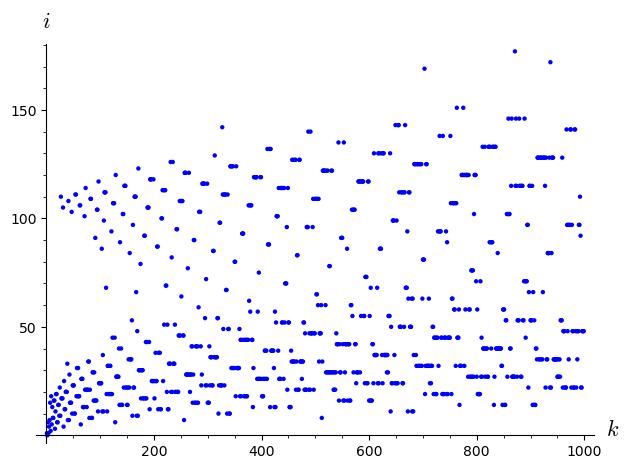
\includegraphics[scale=0.7]{imgs/collatz.png}
  \caption{Tempo de parada $f^i(k) = 1$}
  \label{img:collatz}
\end{figure}
  

Mesmo que você tenha feito tudo certo, não há garantia que
a sua função \ils{collatz} vai eventualmente chegar em um
resultado $i$. Se a conjectura de Collatz for falsa e existir
um contra exemplo, isto é, algum $k_0 \in \NN$ tal que
$f^i(k_0) \neq 1$ para todo $i \in \NN$, então a sua função
será executada por toda a eternidade. Então se você tentou calcular
\ils{collatz(k)} e o seu programa não retornou resultado
alguma das seguintes opções é verdadeira: 1) você cometeu
algum erro no código (esperamos que não), 2) o seu $k$ é
muito grande e o seu computador ainda está no caminho
(o mais provável), ou 3) parabéns, você encontrou um contra
exemplo para a conjectura de Collatz.

Mesmo que a conjectura de Collatz já tenha sido verificada para
números muito muito grandes, não há garantia que ela seja válida.
Um exemplo clássico disso é uma conjectura de Polya, feita
em 1919, sobre
a paridade da quantidade de divisores até certo número. Embora
a afirmação pareça ser válida ao análisar os
primeiros naturais, um contra exemplo foi encontrado na década
de 60. Hoje sabemos que o menor contra exemplo 
para conjectura de Polya é o número $906\,150\,257$.
Assim, ainda que programas de computador forneçam indícios de
que uma afirmação seja verdade, uma demonstração
é essencial para realmente confirmar sua validade.
Por outro lado, se suspeitarmos que uma afirmação é falsa, 
um contra exemplo encontrado computacionalmente
já garante que afirmação não é verdadeira.


\begin{exercise}
  Pesquise sobre a conjectura de Polya e verifique que ela é
  válida para os primeiros $1000$ naturais.
\end{exercise}

\subsection{Primos Gêmeos}
Vejamos uma lista com os 100 primeiros primos
\begin{sageinput}
print(primes_first_n(100))                                                                         
\end{sageinput}
\begin{sageoutput}
[2, 3, 5, 7, 11, 13, 17, 19, 23, 29, 31, 37, 41, 43, 47, 53, 59, 61, 67, 71, 73, 79, 83, 89, 97, 101, 103, 107, 109, 113, 127, 131, 137, 139, 149, 151, 157, 163, 167, 173, 179, 181, 191, 193, 197, 199, 211, 223, 227, 229, 233, 239, 241, 251, 257, 263, 269, 271, 277, 281, 283, 293, 307, 311, 313, 317, 331, 337, 347, 349, 353, 359, 367, 373, 379, 383, 389, 397, 401, 409, 419, 421, 431, 433, 439, 443, 449, 457, 461, 463, 467, 479, 487, 491, 499, 503, 509, 521, 523, 541]
\end{sageoutput}
Analisando atentamente notamos que os primos parecem se distanciar
uns dos outros a medida que crescem, mas, vez ou outra, existem pares de primos
muito próximos, por exemplo: $107$ e $109$, $239$ e $241$, $419$ e $421$, etc. 
Primos $p<q$ são ditos \emph{gêmeos} se $q = p+2$.
\index{Número!primo!gêmeo}
Faça
os exercícios a seguir e crie sua própria conjectura sobre primos gêmeos.
\index{Conjectura!primos gêmeos}

\begin{exercise}
  Crie um código que conte quantos pares de primos gêmeos existem
  até $1000$. E áté $10\,000$? E $100\,000$?
\end{exercise}

Discutiremos mais sobre primos especiais
e a distribuição dos números primos no Capítulo \ref{chap:primos}.

\subsection{Sequências Recorrentes e Expressões Simbólicas}
\label{par:fib}
A sequência de Fibonacci $(u_n)$ é definida da seguinte forma:
\index{Fibonacci}\index{Sequência!de Fibonacci}
$u_0 = u_1 = 1$ e $u_{n} = u_{n-1} + u_{n-2}$ para $n\geq 2$.
Usando a recursividade podemos calcular o valor de $u_n$ de
forma simples
\begin{sageinput}
def fib(n):
  if n == 0 or n == 1:
    return 1
  return fib(n-1) + fib(n-2)
[fib(n) for n in [0..10]]
\end{sageinput}
\begin{sageoutput}
[1, 1, 2, 3, 5, 8, 13, 21, 34, 55, 89]
\end{sageoutput}
De forma mais geral, uma sequência recorrente linear
de ordem $k$ é uma sequência $(x_n)$ tais que existem
constantes $c_1,\cdots,c_k$ tais que
$$
  x_{n+k} = \sum_{j = 1}^k c_j x_{n+k-j}
$$
para $n \in \NN$. Tais sequências dependem dos seus $k$
primeiros termos.

\begin{exercise} 
  Crie um código sage que calcule o valor de uma
  sequência recorrente linear, como a $(x_n)$ acima,
  dados os seus $k$ primeiros
  termos e as constantes $c_j$, $1\leq j \leq k$.
\end{exercise}

Apesar de apresentarmos a sequência de Fibonacci
de forma recursiva, existe uma forma geral para 
os termos $u_n$:
$$
u_n = \frac{\varphi^n - \psi^n}{\varphi - \psi},\quad
\text{ onde }
\varphi = \frac{1+\sqrt{5}}{2}
\text{ e }
\psi = \frac{1-\sqrt{5}}{2}
$$
A existência de uma fórmula desse tipo vale
para sequências recorrentes lineares mais
gerais, recomendamos a leitura de \cite[Apêndice B]{tnumgugu},
especialmente a Seção B.4 (no caso da fórmula
acima para sequência de Fibonacci, você pode
demonstrar a fórmula por indução).
 O código a seguir
calcula o n-ésimo elemento na sequência de Fibonacci
usando essa fórmula geral.
\begin{sageinput}
def fib_g(n):
    phi = (1+sqrt(5))/2
    psi = (1-sqrt(5))/2
    return (phi^n - psi^n)/(phi-psi)  
print(fib_g(5))
\end{sageinput}
O resultado deveria ser \ils{8}, certo? Mas...

\begin{sageoutput}
1/320*sqrt(5)*((sqrt(5) + 1)^6 - (sqrt(5) - 1)^6)
\end{sageoutput}
Se você estiver usando o \sage em algum notebook
(no cocalc, SageMathCell ou  jupyter), pode pedir
para o \sage mostrar o resultado usando a função
\ils{show} ao inves do \ils{print}
\footnote{No interpretador \sage essa
função irá retornar o código \LaTeX\ da
visualização exibida.}, será exibida a expressão

$$
\newcommand{\Bold}[1]{\mathbf{#1}}\frac{1}{320} \, \sqrt{5}
  {\left({\left(\sqrt{5} + 1\right)}^{6} - {\left(\sqrt{5} - 1\right)}^{6}\right)}
$$
O leitor mais corajoso pode verificar que essa expressão
realmente é igual a $8$. No \sage, podemos obter
esse resultando usando a função \ils{expand}:
\begin{sageinput}
expand(fib_g(6))
\end{sageinput}
\begin{sageoutput}
8
\end{sageoutput}
O resultado \emph{inesperado} é na verdade uma das
vantagens do \sage. Em uma linguagem de programação usual,
como no próprio Python, ao definir 
$\varphi = \frac{1+\sqrt{5}}{2}$, o valor seria convertido
em um número real --- na verdade, no ponto flutuante
que aproxima $\varphi$, induzindo um erro de aproximação ---
depois disso as contas são feitas com essas aproximações.
\textbf{O código abaixo está em linguagem Python, e não
\sage} (por isso foi necessário importar a função \ils{sqrt},
no \sage isso não é necessário).
\begin{sageinput}
>>> from math import sqrt
>>> phi = (1+sqrt(5))/2
>>> print(phi)
>>> print(type(phi))
\end{sageinput}
\begin{sageoutput}
1.618033988749895
<class 'float'>
\end{sageoutput}
% Após isso, as contas são feitas usando esse tipo de dado.
No \sage, por outro lado, o cálculo é feito internamente de
forma simbólica.
Vejamos o tipo de dado que é $\varphi$.
\begin{sageinput}
phi = (1+sqrt(5))/2
parent(phi)                                                                                        
\end{sageinput}
\begin{sageoutput}
Symbolic Ring
\end{sageoutput}
Isso significa que, da forma como foi definido,
\ils{phi} é uma \emph{expressão simbólica}. Você
pode visualizar o valor real (aproximado) de 
$\varphi$ com  \ils{RR(phi)}, mas
há muitas vantagens em se usar expressões simbólicas,
mesmo quando estamos trabalhando apenas com números.
Não usaremos a computação simbólica de forma mais
aprofundada nesse texto, mas a ideia é que os
cálculos são feitos de forma mais parecida com o que nós
(humanos) fazemos (afinal, ao fazer uma conta com 
o $\varphi$ você substituiria seu valor por
$\approx 1.61803398874989...$ e usaria esse número?).
Os exercícios a seguir o guiarão por algumas das
possibilidades do cálculo simbólico
\footnote{Algumas das manipulações
que faremos com expressões simbólicas, quando lidam com expressões
polinomiais, são feitas de forma mais eficiente no
\sage usando outro tipo de objeto, elementos
de anéis de polinômios.}.

\begin{exercise}
  Não apenas números podem ser tratados simbolicamente
  pelo \sage mas, principalmente, variáveis. Por padrão
  a única variável (no sentido computacional) que o \sage
  assume ser uma variável (no sentido matemático) é o
  \ils{x}, mas você pode definir outras variáveis.
  \begin{itemize}
    \item[a)] Crie uma variável $y$ com a função \ils{var('y')} \index[sage]{\ils{var}}
    e verifique o seu tipo usando a função \ils{parent}, como
    fizemos acima.
    \item[b)] Defina $f = x^3 - y^3$ e use a função \ils{factor}
    para encontrar a fatoração de $f$ (sim, é o mesmo \ils{factor}
    que fatora um número em primos!)
    \item[c)] É possível substituir valores em uma
    expressão simbólica. Tente \ils{f.subs(x==2,y==1)}. 
    \item[d)] \ils{derivative(f,y)} deve ser autoexplicativo.
    \index[sage]{\ils{derivative}}
    \index[sage]{\ils{.subs}}
    Mude a expressão para $f$ e calcule sua derivada. Usando
    o método \ils{.subs()} é possível calcular a derivada
    em um ponto específico. O que ocorre
    se tentarmos calcular a derivada em um ponto onde a função
    não é diferenciável? (Dica: no sage $|x|$ pode ser escrito
    como \ils{abs(x)})
    \item[d] Desafio: Construa um código que calcule
    (simbolicamente) a derivada
    de uma função
    sem usar a função \ils{derivative}. (Dica: Crie uma
    nova variável \ils{h}, se lembre da definição de
    derivada e use a função \ils{limit}). \index[sage]{\ils{limit}}
  \end{itemize}
\end{exercise}

\begin{exercise} 
  A função \ils{bool()} verifica se o argumento
  passado é verdadeiro ou falso.
  Tente explicar o que está acontecendo no código a seguir:
  \begin{sageinput}
print(bool(sqrt(x^2) == x))
assume(x>0)
print(bool(sqrt(x^2) == x))
  \end{sageinput}
  \begin{sageoutput}
False
True
  \end{sageoutput}
\end{exercise}

\begin{exercise} 
  Uma das mais importantes aplicações do cálculo
  simbólico é a resolução de equações. 
  \begin{itemize}
    \item[a)] Interprete os resultados de
    \ils{solve(x\^{}5-1,x)}  e \ils{solve(x\^{}7+x\^{}2-2*x+2,x)}.
  \end{itemize}
  \index[sage]{\ils{solve}}
  Vamos
  encontrar a interseção entre o círculo unitário
  $x^2 + y^2 = 1$ e a reta $x+2y = 1$.
  \begin{sageinput}
eqs = [x^2 + y^2 == 1, x+2*y == 1]
solve(eqs,x,y)
  \end{sageinput}
  \begin{sageoutput}
[[x == 1, y == 0], [x == (-3/5), y == (4/5)]]
  \end{sageoutput}
  \begin{itemize}
    \item[b)] Encontre os pontos na interseção entre
    as curvas $y^2 = x^3 + x$ e $y = 3x$.
    \item[c)] Você pode verificar se o resultado
    está correto o substituindo nas equações...
    \item[d)] ... ou pode \emph{verificar} visualmente
    exibindo as curvas e os pontos envolvidos. Por exemplo,
    o ponto $(0,0)$ é um ponto na interseção.
    \begin{sageinput}
var('y')
c1 = implicit_plot(y^2 == x^3 + x,(-1,1),(-1,1),color='green') 
c2 = implicit_plot(y == 3*x,(-1,1),(-1,1),color='red')
p = point((0,0),size=40,color='black')
show(c1+c2+p)
    \end{sageinput}
    \begin{figure}[h]
      \centering
      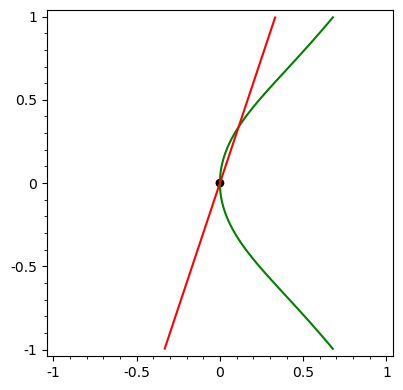
\includegraphics[scale=0.6]{imgs/cepoints.png}
      \caption{Interseção entre $y^2 = x^3 + x$ e $y = 3x$}
      \label{img:cepoints}
    \end{figure}
  \end{itemize}
    O resultado está na Figura \ref{img:cepoints}. Os
    \ils{(-1,1)} representam os intervalos de $x$ e $y$ no gráfico.
    Assim o código \ils{implicit\_plot(eq,(a,b),(c,d))} vai
    \index[sage]{\ils{implicit\_plot}}
    exibir o gráfico da equação implícita nas variáveis $x$ e $y$
    dada em \ils{eq} no retângulo $[a,b]\times[c,d]$, isto é,
    $a\leq x \leq b$ e $c\leq y \leq d$.
    Para uma das soluções do item $d)$ você vai precisar
    alterar o intervalo para conseguir visualizar o ponto.
    \index{Gráfico!Curva implícita}
\end{exercise}

\begin{exercise} 
  Use a técnica apresentada em \cite[B.4]{tnumgugu} para 
  encontrar a fórmula geral da recorrência
  $x_n = 4x_{n-1} + 3x_{n-2} - 14x_{n-3} -6x_{n-4}$ com termos
  iniciais $x_0 = x_1 = 4, x_2 = 22$ e $x_3 = 58$.
\end{exercise}


Apesar de não entrarmos em muitos detalhes, o
cálculo simbólico é uma das ferramentas mais úteis do \sage. 
\index{Cálculo Simbólico}
A documentação oficial possui uma extensa lista de
aplicações, que incluem resolução de equações, cálculos
envolvendo derivadas,
integrais, séries, etc. Veja \cite[Symbolic Calculus]{sagedoc}.




\section{Exercícios}
\begin{exercise} 
  Crie um código \sage que funcione como a função
  \ils{divisors}. Tente otimizar o seu código
  (Veja o item \textit{b)} do Exercício \ref{ex:fatoracaoprimos}).
\end{exercise}

\begin{exercise} 
  \label{ex:fatorial}
  Use a recursividade para criar uma função que calcule o fatorial de
  um número. Siga as instruções:
  \begin{itemize}
    \item[a)] Defina uma função meu\_fatorial com a
    com assinatura \ils{def meu\_fatorial(n):}
    \item[b)] Teste se $n = 0$, nesse caso a função
    deve retornar o valor $1$.
    \item[c)] Se $n>1$, a função deve retornar
    $n\times(n-1)!$, isto é,  \ils{n*meu\_fatorial(n-1)}.
  \end{itemize}
\end{exercise}

\begin{exercise} 
  Use a recursividade para calcular o $\mdc$ entre dois inteiros
  não ambos nulos. Use o Lema \ref{lemma:mdc}.
\end{exercise}

\begin{exercise}
  \label{ex:fatoracaoprimos}
  Reescreva um algoritmo que encontre a fatoração
  de um natural $n>1$ com as otimizações discutidas. Atente
  para os itens a seguir.
  \begin{itemize}
    \item[a)] Remova o uso da recursividade, dessa forma você
    pode criar uma lista \ils{fatores} dentro da própria função
    e armazenar os fatores primos encontrados.
    \item[b)] Prove que se $p$ é o menor primo dividindo
    $n$, então $p \leq \sqrt{n}$. Use esse fato para limitar superiormente
    a busca pelos fatores primos de n.
    \item[c)] Prove que se $p$ é o menor primo dividindo $n$,
    então nenhum primo menor que $p$ divide $n/p$.  Use esse
    fato para limitar inferiormente a busca pelos fatores primos de n.
  \end{itemize}
\end{exercise}

\begin{exercise}
  XGCD de forma mais direta 
\end{exercise}

\begin{exercise}
  O algoritmo de Euclides estendido pode ser descrito na forma
  matricial. Iniciamos com a matriz
  $$M = \begin{pmatrix}
    x_0 & x_1 \\
    y_0 & y_1 \\
    r_0 & r_1
  \end{pmatrix}
  = \begin{pmatrix}
    1 & 0 \\
    0 & 1 \\
    a & b
  \end{pmatrix}.
  $$
  Agora, enquanto $r_1 \neq 0$, tome $q = \lfloor r_0/r_1\rfloor$,
  e alteramos a matriz $M$ da seguinte forma:
  $$
    M \longleftarrow M 
    \begin{pmatrix}
      0 & 1 \\
      1 & -q
    \end{pmatrix}.
  $$
  Verifique que, ao final do processo teremos que $r_0 = \mdc(a,b)$ e
  $x_0a+y_0b = \mdc(a,b)$. 
  Pesquise sobre a manipulação de matrizes no \sage e implemente
  o algoritmo de Euclides estendido da forma descrita acima. (Note que não
  é preciso definir variáveis auxiliares $x_0,x_1,y_0,\dots$, todas as informações
  estão contidas na matriz $M$ e em $q$.)
\end{exercise}

\begin{exercise}
  Dada uma fração contínua $[a_0;a_1,a_2,a_3,\dots]$, sua
  $n$-ésima convergente $p_n/q_n$ pode ser calculada 
  através da relação de recorrência
  % Crie um código que retorne a $n$-ésima convergente $p_n/q_n$ de uma
  % fração contínua $[a_0;a_1,a_2,a_3,\dots]$ usando as relações
  % de recorrência
  $$
  \begin{cases}
    p_n = a_np_{n-1} + p_{n-2} \\
    q_n = a_nq_{n-1} + q_{n-2} \\
  \end{cases}
  $$
  \begin{itemize}
    \item[a)] As relações acima são conhecidas como fórmulas de Wallis.
    Dê uma demonstração usando indução.
    \item[b)] Crie um código que calcule a $n$-ésima convergente
    usando as fórmulas de Wallis. Compare o resultado do seu código
    com o obtido pelo método \ils{.convergent}.
    (Dica: você pode tratar uma fração contínua  como uma lista para obter seus termos,
  por exemplo, \ils{continued\_fraction(pi)[4]} retorna \ilso{292}.)
  \end{itemize}

  
\end{exercise}


\begin{exercise}
  Um bom aluno de álgebra abstrata deve ter notado que existem
  muitas semelhanças entre o anel dos inteiros $\ZZ$ e o anel dos
  polinômios em uma indeterminada com coeficientes em um corpo, por exemplo, $\QQ[t]$.
  Por exemplo, é possível efetuar a divisão euclidiana
  de um polinômio por outro (não nulo), com condições análogas de unicidade,
  você também pode calcular o $\mdc$ entre polinômios, fatorá-los, etc.
  O \sage consegue manipular polinômios tão bem quanto manipula
  os inteiros. Para trabalhar com os polinômios precisamos primeiramente
  definir o ambiente em que eles estão (já que, como os números, 
  um polinômio com a mesma expressão pode ser considerado
  como elemento de vários aneis distintos), sobre os racionais, por
  exemplo, podemos definir $\QQ[t]$ com
  o comando \ils{P.<t>  = QQ[]}. Ao mesmo tempo que
  estamos definindo \ils{P} $= \QQ[t]$, também estamos indicando
  ao \sage que, a partir de agora, \ils{t} deve ser considerado como
  a indeterminada do anel $\QQ[t]$.
  Na célula a seguir definimos o anel
  $\QQ[t]$, e exploramos o polinômio $f(t) = t^6 - 1 \in \QQ[t]$. Não exibimos
  o resultado.
\begin{sageinput}
P.<t> = QQ[t]
f = P(t^6 - 1)
print(f)
print(f(5))
print(f.quo_rem(P(t^2 - 1)))
print(f.quo_rem(P(t^4+2*t)))
print(f.is_irreducible())
print(factor(f))
f.roots()
f.roots(QQbar)
\end{sageinput}
\begin{itemize}
  \item[a)] Execute as funções acima e interprete o resultado. 
  \item[b)] Pesquise por mais funções disponíveis para polinômios.
  \item[c)] Teste a aritmética para polinômios sobre outros anéis.
 \end{itemize}
\end{exercise}

\begin{exercise}
  Pesquise sobre a função \ils{timeit} ou o comando mágico
  \ils{\%timeit}. COMPARAR OS TEMPOS DE EXECUÇÃO
  \index[sage]{\ils{timeit}}
\end{exercise}

% \chapter{Primos}
\label{chap:primos}

No Capítulo \ref{chap:div} vimos as principais ferramentas 
relacionadas aos números primos no \Sage. Nesse capítulo
iremos usar essas e outras ferramentas para explorar propriedades e
resultados importantes sobre primos. Uma referência fundamental para
os aspectos computacionais dos números primos pode
ser vista em \cite{crandall2006prime}
 


\section{Fórmulas que geram?}

\section{Pseudoprimos (Expandir a discussão)}

\subsection{Pseudoprimos de Fermat}


O Pequeno Teorema de Fermat afirma que se $p$ é primo
e $1\leq a<p$, então $a^{p-1}$ deixa resto $1$ na
divisão por $p$. Geralmente esse teorema é apresentado
usando a linguagem de aritmética modular, como veremos
no Capítulo \ref{chap:modular}. 

Podemos usar a contrapositiva desse fato
para concluir que $n$ é composto: basta encontrar  algum $1\leq a< n$
tal que $a^{n-1}$ não deixa resto $1$ na divisão por $n$. A recíproca,
no entanto, não é válida --- existem naturais
$n$ e $1\leq a < n$, tais que $a^{n-1}$ deixa resto
$1$ na divisão por $n$ mas $n$ não é primo. Nesse caso dizemos que
$n$ é pseudoprimo na
base $a$. 

\begin{exercise}
  Usando os métodos \ils{is\_prime} e \ils{quo\_rem}
encontre os $100$ primeiros pseudoprimos de Fermat na base $2$.
\index[sage]{\ils{is\_prime}}
\end{exercise}

\begin{exercise}
  Generalize o seu código do exercício anterior para encontrar
  os $k$ primeiros pseudoprimos de Fermat em uma base $a\geq 2$ 
  arbitrária. (existe um teorema que garante a existência de infinitos
  pseudoprimos de Fermat para qualquer base $a \geq 2$, veja
  \cite[Theorem 3.4.4]{crandall2006prime})
\end{exercise}

\begin{exercise}
  Pesquise sobre números de Carmichael e encontre os $5$ primeiros.
\end{exercise}

Qualquer teorema do tipo ``\emph{se $p$ é primo então $S(p)$}",
onde $S$ é uma afirmação sobre naturais, induz uma noção
de pseudoprimo: Se $n$ é um número composto para
qual a afirmação $S(n)$ é válida, dizemos que $n$ é um
$S$-pseudoprimo. Sendo assim, se a condição $S$ for
fácil de ser verificada, podemos utilizá-la como
um teste de  primalidade probabilístico. Claramente
só nos interessa o caso em que que existem poucos 
$S$-pseudoprimos. Por exemplo, todo primo $p$
satisfaz $S(n)$, onde $S(n)$ é a 
condição \emph{$n$ é igual a $2$ ou é ímpar}, no 
entanto existem muitos pseudoprimos associados a
essa condição com relação aos primos já que
todos os ímpares compostos a satisfazem. 

Dessa forma, teoremas
que indicam a relação entre os pseudoprimos sob
uma condição $S$ e os verdadeiramente primos 
são muito importantes. Há certas propriedades
para as quais não se conhece nenhum pseudoprimo. 
MELHORAR ESSA DISCUSSÃO




\section{Distribuição}

Como discutimos, o estudo do comportamento dos números primos
é um dos principais tópicos de estudo de uma área chamada
Teoria Analítica dos Números. O objeto mais importante
dessa área é, sem dúvida, a função de contagem dos números
primos \index{Função!$\pi$, contagem de primos}
$\pi:\RR_{\geq 0} \to \ZZ_{\geq 0}$ que associa a cada
número real positivo $x$ a quantidade de primos menores
ou iguais a $x$, isto é:
$$
  \pi(x):= \#\{p \in \NN \mid p\text{ primo e } p\leq x\}
$$

Com as funções apresentadas no Capítulo \ref{chap:div}
não deve ser difícil você mesmo criar a sua função $\pi$.
A função $\pi$ implementada no \Sage é chamada de \ils{prime\_pi}.
\index[sage]{\ils{prime\_pi}}
\begin{sageinput}
print("pi(200)\t=", prime_pi(200))
print("pi(6.9)\t=", prime_pi(6.9))
\end{sageinput}
\begin{sageoutput}
pi(200) = 46
pi(6.9) = 3
\end{sageoutput}

Podemos visualizar o gráfico da função $\pi(x)$ através
da ferramenta \ils{plot} do \Sage.
\index[sage]{\ils{plot}}
\begin{sageinput}
plot(prime_pi,10,100)
\end{sageinput}
\begin{figure}[h]
  \centering
  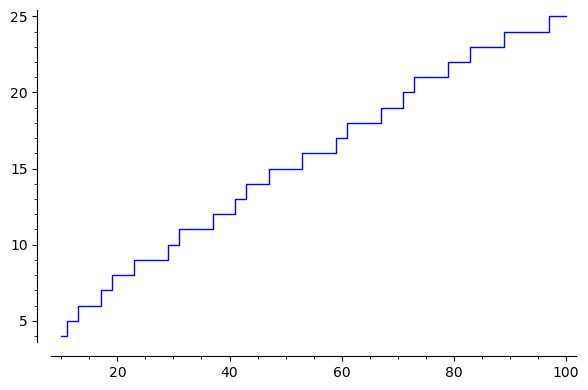
\includegraphics[scale=0.7]{imgs/prime_plot.png}
  \caption{Gráfico de $\pi(x)$}
  \label{img:primeplot}
\end{figure}

Muitos dos resultados sobre o comportamento e a distribuição de primos
são escritos usando a função $\pi(x)$, há um interesse especial em outras
funções reais que aproximam $\pi(x)$. Uma aproximação
em particular, encontrada por Legendre e Gauss e 
provada cerca de um século depois, é tão importante que ganhou
o nome de \emph{Teorema dos Números Primos}.
A hipótese de Riemann 
um dos maiores problemas em aberto na matemática, é equivalente
a certas estimativas sobre o erro na aproximação de $\pi(x)$.
Discutiremos algumas dessas aproximações
mais adiante. Antes disso, vejamos um exemplo mais elementar.
O matemático francês Joseph Bertrand conjecturou em 1845 que
\index{Postulado de Bertrand}
entre um inteiro $n>1$ e seu dobro sempre há um número primo;
isto é, existe um $p$ primo com $n\leq p\leq 2n$. Ora, como
$\pi(2n)$ conta os primos até $2n$ e $\pi(n)$ até $n$,
essa afirmação é equivalente a $\pi(2n)>\pi(n)$, ou seja,
$\pi(2n) - \pi(n) \geq 1$.
Observe na figura \ref{fig:bertrand} o comportamento de
$\pi(2n) - \pi(n)$ para $n$ entre $100$ e $300$.
\begin{sageinput}
def bertrand(n):
    return prime_pi(2*n) - prime_pi(n)
plot(bertrand,100,300,color='black')
\end{sageinput}
\begin{figure}[h]
  \centering
  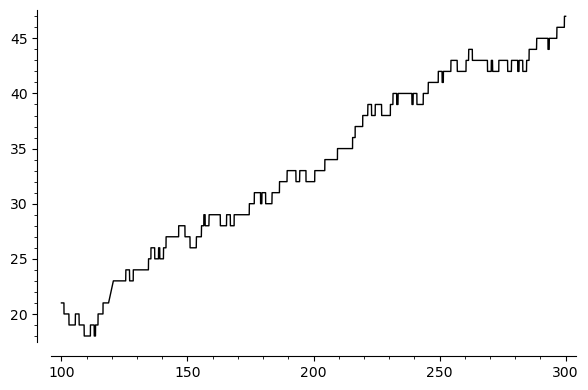
\includegraphics[scale=0.7]{imgs/bertrand.png}
  \caption{$\pi(2n) - \pi(n)$}
  \label{fig:bertrand}
\end{figure}
Observe que, ao contrário de $\pi(n)$, que é naturalmente
não decrescente, ${\pi(2n)-\pi(n)}$ não é monótona. No entanto,
parece ser claro que essa quantidade nunca atinge o valor $1$.
De fato, a conjectura de Bertrand, conhecida como Postulado
de Bertrand, foi demonstrada alguns anos depois pelo matemático
russo Chebyshev. A prova se baseia em estimativas
envolvendo o número binomial ${2n \choose n}$, a suposição
que nenhum primo $p>n$ divide ${2n \choose n}$ implica
em uma cota máxima para $n$. Dessa forma, naturais $n$
maiores que essa cota não satisfazem essa propriedade,
e portanto há um primo $n<p<2n$ e, para naturais menores
que tal cota a afirmação pode ser verificada
computacionalmente, veja \cite[Sec. 5.3]{tnumgugu}.
Diversos outros resultados em teoria dos números são obtidos
de forma similar: prova-se formalmente que o resultado vale 
a partir de determinada constante $K$ e o caso
$n\leq K$ é verificado computacionalmente.
Vale observar que o postulado
de Bertrand pode ser visto como uma consequência direta 
do Teorema dos Números Primos e, como o gráfico 
indica, a quantidade de primos entre $n$ e $2n$
tende a infinito quando $n\to \infty$. 

% teorema dos números primos
\begin{table}
$$
\begin{array}{crrr}
x  & \pi(x) & x/\log(x) & \frac{\pi(x)}{(x/\log(x))} \\ \hline
10  & 4 & 4.34 & 0.92103 \\
10^2  & 25 & 21.71 & 1.15129 \\
10^3  & 168 & 144.76 & 1.16050 \\
10^4  & 1\,229 & 1\,085.74 & 1.13195 \\
10^5  & 9\,592 & 8\,685.89 & 1.10432 \\
10^6  & 78\,498 & 72\,382.41 & 1.08449 \\
10^7  & 664\,579 & 620\,420.69 & 1.07117 \\
10^8  & 5\,761\,455 & 5\,428\,681.02 & 1.06130 \\
10^9  & 50\,847\,534 & 48\,254\,942.43 & 1.05373 \\
10^{10}  & 455\,052\,511 & 434\,294\,481.90 & 1.04780 \\
10^{11}  & 4\,118\,054\,813 & 3\,948\,131\,653.67 & 1.04304 \\
10^{12}  & 37\,607\,912\,018 & 36191\,206\,825.27 & 1.03915 \\
10^{13}  & 346\,065\,536\,839 & 334\,072\,678\,387.12 & 1.03590 \\
\end{array}
$$
\caption{$\pi(x)$, $x/\log(x)$  seu quociente}
\label{tab:tnplog}
\end{table}

$$
  \lim_{x \to \infty}
    \frac{\pi(x)}{\left(\frac{x}{\log x}\right)} = 1
$$

Usamos a notação $\pi(x) \sim \frac{x}{\log x}$

Podemos interpretar o limite acima como a afirmação
que, para $x$ grande, a probabilidade de que um
inteiro menor que $x$ seja primo, isto é, $\pi(x)/x$,
é aproximadamente $1/\log{x}$

\section{Primos em PA}


\section{Funções Aritméticas}
\label{sec:funarit}
 
Chamamos de \emph{função aritmética} uma função da forma
\index{Função!Aritmética}
$f:\NN \to \CC$, nesse texto estudaremos
exclusivamente funções aritméticas cujo contra domínio
é o conjunto dos reais. Gostaríamos que as funções aritméticas 
expressassem propriedades aritméticas sobre os inteiros, para
isso vamos definir mais duas propriedades sobre funções aritméticas:

\begin{itemize}
  \item  Uma função $f:\NN \to \RR$ é dita multiplicativa se
  $f(ab) = f(a)f(b)$ sempre que $a,b \in \NN$ forem coprimos.
  \item  Uma função $f:\NN \to \RR$ é dita completamente
  multiplicativa se $f(ab) = f(a)f(b)$ para quaisquer $a,b \in \NN$.
\index{Função!Multiplicativa}
\end{itemize}

Já introduzimos implicitamente uma importante função
aritmética. Ao discutirmos números perfeitos falamos
sobre a soma dos divisores de um inteiro e usamos a soma
da lista gerada pela 
função \ils{divisors}. Defina \index{Função!Sigma $\sigma$}
$\sigma:\NN \to \RR$ dada por $\sigma(n) =$ soma
dos divisores positivos de $n$. Representamos
matematicamente essa soma por $\sigma(n) = \sum_{d\mid n} d$. Note que
embora não esteja explicito no somatório, somamos apenas os
divisores positivos.

No \sage a função 
$\sigma(n)$ pode ser calculada usando
\ils{sum(divisors(n))}. Como, ao definir números perfeitos,
consideramos apenas os divisores positivos próprios,
isto é, diferentes de $n$, podemos redefinir números
perfeitos como naturais $n$ satisfazendo $\sigma(n) = 2n$.

A função $\sigma$ pode ser generalizada da seguinte forma:
para $k\geq 0$ inteiro, defina $\sigma_k:\NN \to \RR$
por $\sigma_k(n) = \sum_{d\mid n} d^k$, de forma
que $\sigma_1 = \sigma$. 
Se $k=0$ então
$\sigma_0(n) = \sum_{d \mid n} 1 = $ quantidade de divisores
positivos de $n$, essa função também é denotada por $d(n)$ ou
$\tau(n)$ (não confundir com a função $\tau$ de Ramanujan).

\begin{exercise}  \label{ex:sigma}
  Usando a função \ils{divisors}, crie um código
  que calcule $\sigma_k(n)$ para $k$ e $n$ dados. Usando a
  compreensão de listas isso pode ser feito em apenas uma linha.
\end{exercise}  

O \sage já possui as funções $\sigma_k$ implementadas: $\sigma_k(n)$
pode ser calculado com \ils{sigma(n,k)}, sendo o segundo argumento
\index[sage]{\ils{sigma}}
opcional e tomado como $k=1$ se ausente, isto é, \ils{sigma(n)}
irá retornar $\sigma_1(n) = \sigma(n)$\footnote{Se,
ao resolver o exercício acima, você criou uma função com o nome \ils{sigma},
então ela sobrescreveu a do \sage. Para recuperar a função original basta
reiniciar o sage, reiniciando o kernel se estiver executando um notebook.}
. No entanto, o \sage não
calcula o valor de $\sigma_k$ de forma como fizemos no exercício
\ref{ex:sigma} --- para os mais corajoso, digite \ils{sigma??} e 
tente encontrar o pedaço do código onde a função é realmente calculada.
Isso será justificado após o exercício a seguir:

\begin{exercise}
  Crie um código que escolha pares de naturais $a$ e $b$ coprimos
  aleatórios, calcule $\sigma_k(a)$, $\sigma_k(b)$ e $\sigma_k(ab)$ e
  compare $\sigma_k(a)\sigma_k(b)$ com $\sigma_k(ab)$. Após se convencer
  que $\sigma_k$ é multiplicativa prove esse fato. (Dica: Prove primeiramente
  que se $a$ e $b$ são coprimos e $D_n$ representa o conjunto dos divisores
  positivos de $n$, então existe uma bijeção $D_{a}\times D_{b} \to D_{ab}$).
\end{exercise}


Considere agora um natural $n>1$ e uma função multiplicativa $f$. Se
a fatoração em primos de $n$ é dada por $n=p_1^{e_1} \dots p_r^{e_r}$,
então, como $f$ é multiplicativa
$$
  f(n) = f(p_1^{e_1} \cdots p_r^{e_r}) = f(p_1^{e_1}) \cdots f(p_r^{e_r}),
$$
ou seja, $f$ depende apenas do comportamento nas potências de primos.
Assim, para calcular $f(n)$ onde $f$ é uma função multiplicativa, basta
conhecer os valores de $f$ nas potências de primos e a fatoração em primos
de $n$. 

\paragraph{Função $\varphi$ de Euler}
Uma das funções aritméticas mais importantes é a função $\varphi$ de Euler,
definida da seguinte forma:
$$
  \varphi(n) = \#\{1\leq a \leq n \mid \mdc(a,n) = 1\}
$$
\index{Função!$\varphi$ de Euler}
Para uma potência de primo, digamos $p^e$, $\varphi(p^e)$ conta
os coprimos com $p^e$. Como o único divisor primo de $p^e$  é o próprio
$p$, contamos quantos naturais $1\leq a \leq p^e$, não são divisíveis por
$p$. Existem $p^{e-1}$ multiplos de $p$ menores que $p^e$, portanto
$\varphi(p^e) = p^2 - p^{e-1}$. No \sage, a função de Euler é
implementada na função \ils{euler\_phi}. \index[sage]{\ils{euler\_phi}}

\begin{exercise}
Repita a parte inicial do exercício \ref{ex:sigma}. A demonstração da
multiplicatividade de $\varphi$ exige alguns resultados auxiliares.
Voltaremos a discutir essa função no capítulo \ref{chap:modular}.
\end{exercise}

Como mencionamos, uma função aritmética multiplicativa depende
apenas dos seus valores nas potências de primos. Isso permite
criar funções aritméticas multiplicativas de forma simples,
basta definirmos a função em cada potência de primo $p^e$
e, para um $n \in \NN$ qualquer, basta expandir a definição
usando a multiplicatividade. Note, no entanto, que a condição
de multiplicatividade implica $f(a) = f(a\times 1)= f(a)f(1)$,
portanto $f(1) = 1$ ou $f(a) = 0$ para todo $a \in \NN$.

\begin{example}
  Nesse exemplo implementamos a função aritmética multiplicativa dada por
  $\psi(p^e) = p^e + p^{e-1}$ se $e >0$ e $\psi(1) = 1$.
  Primeiramente criamos a função \ils{psi\_pp} para calcular $\psi$ apenas
  nas potências de primos.
\begin{sageinput}
def psi_pp(n):
    fatoracao = factor(n)
    if len(fatoracao) != 1:
        return "Erro: {} nao potencia de primo".format(n)
    p = fatoracao[0][0]
    e = fatoracao[0][1]
    return p^e + p^(e-1)
    
print("psi(16) =", psi_pp(16))
print("psi(22) =", psi_pp(22))
\end{sageinput}
\begin{sageoutput}
psi(16) =  24
psi(22) =  Erro: 22 nao potencia de primo
\end{sageoutput}
A função \ils{psi} abaixo agora calcula o valor de $\psi(n)$ para
qualquer $n$.
\begin{sageinput}
def psi(n):
    if n <= 0:
        return "Erro: n deve ser positivo"
    if n == 1:
        return 1
    fatoracao = factor(n)
    total = prod([psi_pp(p^e) for (p,e) in fatoracao])
    return total

[psi(i) for i in [1..20]]
\end{sageinput}
\begin{sageoutput}
[1, 3, 4, 6, 6, 12, 8, 12, 12, 18, 12, 24, 14, 24, 24, 24, 18, 36, 20, 36]
\end{sageoutput}
A função \ils{psi} que definimos acima é a função $\psi$ de Dedekind
e tem conexões com a teoria de formas modulares\footnote{A função $\psi$
de dedekind também já está implementada no \sage, mas é necessário
importá-la usando \ils{from sage.arith.misc import dedekind\_psi}.
Na verdade, ao chamar nossa função de \ils{psi}
sobrescrevemos uma função já existente no \sage, chamada
função digamma.}.
\end{example}



\begin{exercise}
Listamos a seguir algumas das principais funções aritméticas.
Para cada uma delas crie um código que calcule tais funções em
um $n$ dado, como fizemos com a função $\psi$ acima. Usamos 
a seguinte notação, se $n \in \NN$ e $n = p_1^{e_1} \cdots p_r^{e_r}$
é a sua fatoração em primos, então
$\omega(n) = r$ e $\Omega(n) = e_1+e_2+\cdots+e_n$. 
Conjecture quais dessas funções são (completamente) multiplicativas
ou (completamente) aditivas. Você consegue provar alguma dessas afirmações?
\begin{table}
\centering
{\renewcommand{\arraystretch}{2.4}
  \begin{tabular}{|l|l|} \hline
    Função & Definicao \\ \hline \hline
    $\mu$ de Möbius & $\mu(n) = 
      \begin{cases}
        (-1)^{\omega(n)} & \text{ se } \omega(n) = \Omega(n) \\ 
        0 & \text{ se } \omega(n) \neq \Omega(n) \\
      \end{cases}$ \\ \hline
    $\lambda$ de Liouville & $\lambda(n) = (-1)^{\Omega(n)}$ \\ \hline
    Soma de Ramanujam &
      $c_q(n) = \sum_{\stackrel{1 \leq a \leq q}{\mdc(a,q) = 1}}
          e^{2\pi i \frac{a}{q}n}$ \\ \hline
    Ordem $p$-ádica & $v_p(n) = \max\{k \geq 0 \mid p^k \mid n\}$ \\ \hline
    von Mangoldt  & $\Lambda(n) = 
    \begin{cases}
      \log(p) & \text{ se } n = p^k \\
      0 & \text{ caso contrário }
    \end{cases}$ \\ \hline
  \end{tabular}}
  \caption{Funções Aritméticas}
  \label{tab:funarit}
\end{table}
\end{exercise}



\newpage
\section{Explore!}
\label{sec:exploreprimos}
\subsection{Primos de Mersenne, GIMPS}

\subsection{Mais conjecturas: Opperman}

\begin{itemize}
  \item Primos especiais (de sophie  germain,etc)
\end{itemize}

\section{Exercícios}

\begin{exercise}
  Construa um código \Sage que crie a Tabela \ref{tab:tnplog}.
\end{exercise}

\begin{exercise}
    Seja $n \in \NN$ e considere a sequência $s_k$ de naturais dada por
    $s_0 = n$ e $s_k = \sigma(s_{k-1}) - s_{k-1}$.
    % terminando a sequência se ela chega no $1$, já que
    % a $\sigma(1) = 1$, ou se a sequência se repete, ou seja,
    % se $s_k = s_l$ para algum $l<k$, nesse caso dizemos
    % que a sequência tem comprimento $k$, nesse caso dizemos
    % que a sequência termina em um ciclo de comprimento $k-l$.
    Por exemplo, para $n = 12$,
    $(s_k) = (12,16,15,9,4,3,1,1,1,\dots)$, 
    para $n = 6$, $(s_k) = (6,6,6,\dots)$.
    As sequências $(s_k)$ são chamadas de \emph{sequência de alíquota}
    \index{Sequência!de alíquota}.
    \begin{itemize}
      \item[a)] Crie um código que calcule a sequência de alíquota
      até um índice dado; isto é, o seu programa deve receber
      $n$ e $i$ e retornar $(s_0,s_1,\dots,s_i)$.
      \item[b)] Prove que a sequência é eventualmente
      constante se chega em algum número perfeito.
      \item[c)] Prove que a sequência termina em um
      ciclo de comprimento $2$ se chega em algum número
      amigável.
      \item[d)] Naturais cuja sequência de alíquota são ciclos
      de comprimento maior que $2$ são ditos \emph{sociáveis}. Encontre o menor
      número sociável $n$ cuja sequência de alíquota
      é um ciclo de comprimento $4$. {\color{red}(verificar, talvez demore muito)}
        %Segundo Wikipedia, 1,264,460 
      \index{Número!Sociável}
      \item[e)] Repita o item anterior para um ciclo de comprimento
        {\color{red}(verificar, talvez demore muito)}
        $5$. %Segundo Wikipedia, 12,496 
      \item[f)] Um número é dito intocável
      \index{Número!Intocável} se não está em nenhuma sequência de alíquota,
      exceto a iniciada por ele, ou seja, não é a soma dos divisores próprios
      de nenhum outro natural. Encontre os $5$ primeiros números
      intocáveis.
    \end{itemize}
\end{exercise}


\begin{exercise}
  Dadas duas funções aritméticas $f,g$, definimos o produto ou
  convolução de Dirichlet de $f$ e $g$ como a função aritmética $h$
  dada por 
  $$
    h(n) = \sum_{d \mid n} f(d) g\left(\frac{n}{d}\right)
  $$
  A notação para convolução de Dirichlet é $f*g$.
  \begin{itemize}
    \item[a)] Prove que se $f$ e $g$ são multiplicativas
    então $f*g$ também é multiplicativa.
    \item[b)] Crie um código que calcule a convolução de Dirichlet
    de duas funções aritméticas dadas.
  \end{itemize}
\end{exercise}
% \chapter{Aritmética Modular}
\label{chap:modular}


\section{A congruência módulo $m$}

Dado $m\in \NN$ fixado, dois inteiros $a$ e $b$ são
ditos \emph{congruentes} módulo $m$ se $m \mid b-a$. Denotamos
\index{Congruência módulo $m$}
essa relação por $a \equiv b \pmod m$.

\begin{example}\label{ex:modbas}
  $137 \equiv 61 \pmod{19}$ pois $19 \mid 137-61 = 76 = 4\times 19$,
  mas também $137 \equiv 4 \pmod{19}$ pois $137-4 = 133 = 7\times 19$.
  Também podemos usar números negativos: $-19 \equiv 2 \pmod 3$
  pois $3 \mid -19 - 2 = -21 = 3 \times (-7)$.
\end{example}

Relembramos as principais propriedades sobre a congruência
e a aritmética modular na proposição a seguir. As demonstrações
podem ser encontradas em \cite[Lema 1.1]{tnumgugu}.
\begin{proposition}\label{prop:prarit}
  Sejam $m \in \NN$, $a,b,c,d \in \ZZ$. Valem as propriedades
  a seguir:
  \begin{itemize}
    \item[i)] $a \equiv a \pmod m$,
    \item[ii)] Se $a \equiv b \pmod m$, então $b \equiv a \pmod m$,
    \item[iii)] Se $a\equiv b \pmod m$ e $b \equiv c \pmod m$, então
    $a \equiv c \pmod m$.
    \item[iv)] Se $a\equiv b \pmod m$ e
        $c \equiv d \pmod m$, então $a+c \equiv b+d\pmod m$
    \item[v)] Se $a\equiv b \pmod m$ e $c \equiv d \pmod m$,
        então $ac \equiv bd\pmod m$
  \end{itemize}
\end{proposition}

As três primeiras propriedades implicam que a congruência
módulo $m$ é uma relação de equivalência, enquanto as últimas duas
dizem que a congruência módulo $m$ respeita a aritmética.

Se $a = qm +r$ é a divisão euclidiana de $a$ por $m$,
então $m \mid a-r$ e portanto $a\equiv r \pmod m$. Assim, dois
números com o mesmo resto na divisão por $m$ são congruentes.
É um exercício simples verificar que a recíproca também
vale; isto é, se $a \equiv b\pmod m$ então $a$ e $b$ deixam
o mesmo resto na divisão por $m$. Esses resultados
implicam que podemos trabalhar com congruência
módulo $m$ nos limitando aos possíveis restos 
da divisão por $m$: $0,1,2,\cdots,m$. Esse é um
fato importante ao se trabalhar com aritmética modular
no \sage.

% Considere a divisão euclidiana de $a$ e $b$ por $m$, 
% digamos $a = q_1m+r1$ e $b = q_2m+r_2$. Note que se $a$ e $b$
% deixam o mesmo, isto é, $r_1 = r_2$, então $b-a = (q_2-q_1)m$,
% portanto $m \mid b-a$, logo $a \equiv b \pmod m$.
% A  recíproca também é válida: se $a \equiv b \pmod m$, então
% $m \mid b-a = (q_2-q_1)m + (r_2-r_1) \therefore m\mid r_2 - r_1$
% e, como $0\leq r_1,r_2 < m$ devemos ter $r_1 = r_2$. Também
% é óbvio que todo número é equivalente.

O $\Sage$ tem diversas ferramentas para se trabalhar com aritmética modular.
A forma mais primitiva é usar o operador \ils{\%} do próprio Python; a
expressão \ils{a \% m} retorna o resto da divisão de $a$ por $m$,
o resultado é, como vimos acima, congruente a $a$ módulo $m$.

\begin{sageinput}
3 % 2
\end{sageinput}
\begin{sageoutput}
1
\end{sageoutput}

O operador \ils{\%} deve ser usado com cuidado pois é um operador
que retorna um inteiro da classe \ils{Integer} (ou \ils{int} no Python),
de forma que \ils{3 \% 5 == 11 \% 8} retorna \ilso{True}, no entanto,
da forma como definimos, $3 \pmod 5 = 11 \pmod 8$ não faz sentido. Além
disso, o \ils{\%} é um operador binário, então devemos
ter cautela ao pensar em \ils{\% m} como um $\pmod m$ no final
de uma expressão: não podemos escrever, por exemplo,
$2 + 2 \pmod 3$ como \ils{2 + 2 \% 2}. Teste e veja o resultado!

Na prática existe outra forma de se trabalhar com aritmética
modular no \sage, a função \ils{mod} e o método \ils{.mod},
que funcionam de formas ligeiramente distintas.
Vejamos alguns exemplos, compare com os resultados do Exemplo
\index[sage]{\ils{.mod}} \index[sage]{\ils{mod}}
\ref{ex:modbas}:
\begin{sageinput}
mod(137,19)
mod(137,19) == mod(4,19)
(-19).mod(3)
\end{sageinput}
\begin{sageoutput}
4
True
2
\end{sageoutput}

Note que, quando $m>0$, tanto o \ils{mod} quanto o \ils{\%}
retornam o resto (se $m<0$ o comportamento do \ils{\%} 
é diferente). Existe uma diferença fundamental entre
no resultado da função \ils{mod}. Enquanto o método \ils{.mod}
e o operador \ils{\%} retornam um número inteiro, o resultado
da função \ils{mod} é um \emph{inteiro módulo $m$}.
\begin{sageinput}
parent(mod(5,13))
\end{sageinput}
\begin{sageoutput}
Ring of integers modulo 13
\end{sageoutput}

\paragraph{Inteirmos módulo $m$} 
O tipo de objeto retornardo pela função \ils{mod} é chamado
de \emph{inteiro módulo $m$}. A ideia é que, como todo
inteiro é congruente a um dos restos $0,1,\dots,m-1$ módulo $m$
podemos \emph{ignorar} os demais inteiros e trabalhar apenas
com os restos, identificando os inteiros fora desse intervalo
com seu resto na divisão por $m$. Formalmente, o que estamos
usando é o fato da congruência ser uma
\emph{relação de equivalência}, \index{Relação de equivalência}
de acordo com as três primeiras propriedades da Proposição
\ref{prop:prarit}. O conjunto dos inteiros módulo $m$ seria
portanto o conjunto quociente de $\ZZ$ por essa relação
de equivalência. Em geral denotamos tal conjunto por
$\ZZ_m$ ou $\ZZ/m\ZZ$. No \sage, podemos definir
o conjunto dos inteiros módulo $m$ usando a função \ils{Zmod},
outro nome para essa função é  \ils{IntegerModRing}.
A seguir definimos $\ZZ_7$ e listamos seus elementos.
\index[sage]{\ils{Zmod}} \index[sage]{\ils{IntegerModRing}}
\begin{sageinput}
ZZ7 = Zmod(7)
print(ZZ7)
print(list(ZZ7))
\end{sageinput}
\begin{sageoutput}
Ring of integers modulo 7
[0, 1, 2, 3, 4, 5, 6]
\end{sageoutput}
Apesar de serem exibidos como inteiros, formalmente
os elementos de $\ZZ_m$ são 
classes de equivalência, em geral
denotados por $[k]$, $\bar k$ ou $k + m\ZZ$,
e a comparação com o \ils{==} desses elementos é,
na verdade, a congruência $\cdot \equiv \cdot \pmod m$.
 Para manipular inteiros como
elementos desse conjunto podemos usar a coerção:
\begin{sageinput}
ZZ3 = Zmod(3)
a = 13
b = ZZ3(a)
print(a, parent(a))
print(b, parent(b))
\end{sageinput}
\begin{sageoutput}
13 Integer Ring
1 Ring of integers modulo 3
\end{sageoutput}

A linha $3$ tem o mesmo efeito de \ils{b = mod(a,3)}.
A aritmética entre elementos de $\ZZ_m$ funciona como 
esperado pela congruência módulo $m$, podemos
fazer as operações tanto usando a coerção para \ils{Zmod(m)}
ou usando o \ils{mod}
\begin{sageinput}
ZZ7 = Zmod(7)
(a,b) = (4,5)
print("Usando o mod:", mod(a,7) + mod(b,7))
print("Usando a coercao:", ZZ7(a) + ZZ7(b))
print("Sao iguais:", mod(a,7) + mod(b,7) == ZZ7(a) + ZZ7(b))
\end{sageinput}
\begin{sageoutput}
Usando o mod: 2
Usando a coercao: 2
Sao iguais: True
\end{sageoutput}
E, de fato, $4 + 5 \equiv 2 \pmod 7$ \footnote{E se você
fizesse a conta usando \ils{mod(a+b,7)}? O resultado seria
o mesmo! Na verdade, esse fato é essencial ao trabalharmos
com $\ZZ_m$, já que garante que a soma herdada dos inteiros
está \emph{bem definida}, o que permite trabalhar com
$\ZZ_m$ como um grupo.}.
Se, ao invés de usar o \ils{mod} ou a coerção tívessemos
usado o método \ils{.mod} ou o operador \ils{\%}, 
os objetos retornados seriam diferentes, no entanto,
ao compará-los com o \ils{==} o resultado seria verdadeiro
, por exemplo, \ils{mod(3,7) == 3 \% 7} retorna \ilso{True}
\footnote{Para os conhecedores de Python: Isso também
é feito no Python, por exemplo, \ils{float(1) == int(1)}
retorna \ilso{True}}. No entanto os métodos disponíveis
para os dois resultados são bastante distintos.

Como há apenas uma quantidade finita de elementos em cada
$\ZZ_m$, podemos listar o resultado de todas as somas possíveis
entre seus elementos. Isso pode ser feito usando o
o método \ils{.addition\_table}.
\index[sage]{\ils{.addition\_table}}
\begin{sageinput}
ZZ7 = Zmod(7)
ZZ7.addition_table(names='elements')                                                               
\end{sageinput}
\begin{sageoutput}
+  0 1 2 3 4 5 6
 +--------------
0| 0 1 2 3 4 5 6
1| 1 2 3 4 5 6 0
2| 2 3 4 5 6 0 1
3| 3 4 5 6 0 1 2
4| 4 5 6 0 1 2 3
5| 5 6 0 1 2 3 4
6| 6 0 1 2 3 4 5
\end{sageoutput}
O parâmetro opcional \ils{names='elements'} serve para
exibir o resultado de forma mais natural, tente retirá-lo
e interpretar o resultado. Ao usar
a função \ils{show} para exibir o resultado, obtemos a 
Tabela \ref{tab:Z7}

\begin{table}[h]
$$
\newcommand{\Bold}[1]{\mathbf{#1}}{\setlength{\arraycolsep}{2ex}
\begin{array}{r|*{7}{r}}
\multicolumn{1}{c|}{+}&0&1&2&3&4&5&6\\\hline
{}0&0&1&2&3&4&5&6\\
{}1&1&2&3&4&5&6&0\\
{}2&2&3&4&5&6&0&1\\
{}3&3&4&5&6&0&1&2\\
{}4&4&5&6&0&1&2&3\\
{}5&5&6&0&1&2&3&4\\
{}6&6&0&1&2&3&4&5\\
\end{array}}
$$
\caption{Tabela de adição do $\ZZ_7$}
\label{tab:Z7}
\end{table}

\begin{exercise}
\label{ex:grupoz7}
  Observe, da Tabela \ref{tab:Z7}, que: \textbf{1)} o $0$ é um
  elemento neutro para a adição, isto é,
  $0 + a \equiv a + 0 \equiv a \pmod 7$; \textbf{2)} para todo
  $a \in \ZZ_7$, existe um $b \in \ZZ_7$ tal que $a+b \equiv b+a \equiv 0
  \pmod 7$, em outras palavras, todo elemento tem um
  inverso aditivo em $\ZZ_7$; e \textbf{3)} a soma
  em $\ZZ_7$, sendo herdada de $\ZZ$, é associativa.
  Verifique que essas três propriedades valem para todo
  os conjuntos $\ZZ_m$. Dizemos que $\ZZ_m$ é um \emph{grupo}
  \index{Grupo}
  com a adição módulo $m$.
\end{exercise}



Uma das aplicações da aritmética modular é obter
informações sobre problemas envolvendo números inteiros
o analisando
em um ambiente onde há finitas possibilidades a serem
testadas.A ideia
é que, se alguma igualdade vale entre expressões
envolvendo inteiros, então ela também vale quando
reduzimos a expressão módulo $m$.  Vejamos um exemplo
em que a aritmética
modular resolve uma equação diofantina. 

\begin{example}
 Considere
  a equação $x^2 + y^2 = 4xy + 3$. 
  No entanto, suponha que exista uma solução $(x,y)$ para tal equação,
  devemos ter, portanto, $x^2 + y^2 \equiv 4xy + 3 \pmod 4$.
  Analisemos os casos, sabemos que existem $4$ restos possíveis
  para um inteiro na divisão por $4$, assim $x \equiv 0,1,2
  \text{ ou } 3 \pmod 4$, portanto $x^2 \equiv 0^2, 1^2, 2^2
  \text{ ou }  3^2 \pmod 4$, assim $x^2 \equiv
  \pmod 4$. De forma análoga $y^2 \equiv  0 \text{ ou } 1 \pmod 4$,
  assim, para o lado esquerdo, temos
  $$
    x^2 + y^2 \equiv (0 \text{ ou } 1) + (0 \text{ ou } 1) \equiv 0, 1
    \text{ ou } 2 \pmod 4
  $$
  Por outro lado, no lado direito, como $4xy$ é múltiplo de $4$,
  temos que $4xy \equiv 0 \pmod 4$, assim
  $$
    4xy + 3 \equiv 3 \pmod 4
  $$
  Como $3 \not \equiv 0, 1 \text{ ou } 2 \pmod 4$ concluímos que
  a suposta solução não pode existir. Assim, $x^2 + y^2 = 4xy + 3$
  não possui soluções em $\ZZ$. Essa equação define uma
  hipérbole em no plano real, o que provamos é que não há
  nenhum ponto nessa hipérbole com ambas as coordenadas inteiras.
\end{example}

Ainda que a análise de uma
equação módulo $m$ não produza uma inconsistência
que permita concluir a não existência de soluções, como acima,
por vezes podemos
subtrair dela alguma informação (veja o exercício \ref{ex:ecdiofcong}).

Vale destacar que, no caso geral, 
a análise da equação módulo $m$ não resolve completamente
o problema: 
existem equações que possuem soluções módulo $m$ para todo $m$
mas não possuem soluções inteiras. 
O procedimento de analisar soluções para equações nos inteiros
estudando as reduções módulo $m$ é estudado pelo Princípio
de Hasse, veja \cite{aitken2011counterexamples} para
uma descrição detalhada.

\section{Invertíveis módulo $m$}
\label{sec:invmodm}
Voltamos às propriedades da aritmética modular. Note que
não há, na Proposição \ref{prop:prarit}, uma propriedade análoga ao
\emph{cancelamento} que é permitido para
números inteiros: se $ac = bc$ com $c \neq 0$, então
$a = b$. Essa propriedade não á válida em geral na aritmética
modular, por exemplo
$$
  4\times 3  = 12 \equiv 0 \equiv 18 = 3\times 6 \pmod 6
\text{ mas } 4 \not\equiv 6 \pmod 6
$$
ou seja, não podemos
cancelar o $3$ em ambos os lados da congruência. Em alguns
casos o cancelamento pode, de fato, ser feito. A proposição
a seguir mostra o caso geral, a demonstração
fica a cargo ao leitor.

\begin{proposition}
  Sejam $a,b,c \in \ZZ$ e $m \in \NN$. Se $ac \equiv bc
  \pmod m$, então $a \equiv b \pmod{\frac{m}{d}}$, onde
  $d = \mdc(m,c)$. Em particular, se $\mdc(m,c) = 1$,
  então $a \equiv b \pmod m$.
\end{proposition}

A validade de cancelar um $c$ numa equação em
congruência está intimamente ligado com o
conceito de invertível módulo $m$.  Dizemos que
$c \in \ZZ$ é invertível módulo $m$ se existe $c' \in \ZZ$
tal que $cc' \equiv 1 \pmod m$.  O inteiro
$c'$ é dito \emph{inverso} de $c$ módulo $m$.
\index{Inverso módulo $m$}
Por exemplo,
$c = 3$ é invertível módulo $4$ pois $c' = 3$
satisfaz $cc' = 3\times 3 \equiv 9 \equiv 1 \pmod m$.
Por outro lado $2$ não é invertível módulo $4$ (verifique isso!).

Verifiquemos se $7$ é invertível módulo $11$. 
Para isso basta calcular $7d \pmod{11}$ para todos
os resíduos $d$ módulo $11$ possíveis:
\begin{sageinput}
c = 7
for d in [0..10]:
  print("7*{} = ".format(d), mod(c*d,11), "mod 11")
\end{sageinput}
\begin{sageoutput}
7*0 =  0 mod 11
7*1 =  7 mod 11
7*2 =  3 mod 11
7*3 =  10 mod 11
7*4 =  6 mod 11
7*5 =  2 mod 11
7*6 =  9 mod 11
7*7 =  5 mod 11
7*8 =  1 mod 11
7*9 =  8 mod 11
7*10 =  4 mod 11
\end{sageoutput}
Como $7\times 8 \equiv 1 \pmod{11}$, temos que $7$ é invertível
módulo $11$. Implemente o caso geral no exercício a seguir.

\begin{exercise}
\label{ex:invers}
  Crie um código que encontre, usando a definição,
  todos os invertíveis módulo um $m$ dado (Para cada $c$,
  percorra todos os resíduos possíveis $d = 0, 1, \dots, m-1$,
  verificando se $cd \equiv 1 \pmod m$). 
  \begin{itemize}
    \item[a)] Teste o seu código para alguns valores distintos de $m$. 
    \item[b)] Se um $c$ é invertível módulo $m$, quantas
    inversas ele possui?
    \item[c)] Você consegue encontrar algum padrão
    nos invertíveis módulo $m$, $m$ fixo?
    \item[d)] Você consegue encontrar algum padrão na quantidade
    de invertíveis módulo $m$? Teste primeiramente valores primos
    para $m$, e,  em seguida, potências de primos.
    \item[e)] Use o método \ils{.multiplication\_table}
    para exibir a tabela de multiplicação do anel de inteiros módulo
    $m$, como fizemos com a adição.
  \end{itemize}
\end{exercise}

A busca por invertíveis e inversas que implementamos
através da força bruta no exercício anterior pode ser
reduzida a um calculo já conhecido nosso.

\begin{proposition}
\label{prop:inversa}
  Seja $m \in \NN$ fixado. Um inteiro $c \in \ZZ$ é
  invertível módulo $m$ se e somente se $\mdc(a,m) = 1$.
  Além disso, se $x,y \in \ZZ$ são tais que
  $cx+my = 1$, então $x$ é uma inversa para $c$
  módulo $m$.
\end{proposition}
\begin{proof}
  Pelo Teorema \ref{thm:bezout}, se $c$ e $m$ são coprimos,
  existem $x,y \in \ZZ$ tais que $cx + my = 1$, reduzindo
  essa igualdade módulo $m$ temos que $cx \equiv 1 \pmod m$,
  portanto $c$ é invertível módulo $m$ e $x$ é sua 
  inversa. Por outro lado, se $c$ é invertível módulo $m$ 
  existe $c' \in \ZZ$ tais que $cc' \equiv 1 \pmod m$, portanto
  $m \mid cc' - 1$, logo existe $k \in \ZZ$ tal que
  $km = cc' - 1 \therefore cc' - km = 1$. Suponha agora
  que $\mdc(m,c)\neq 1$,
  então existe um primo $p$ tal que $p\mid c$ e $p\mid m$,
  portanto $p \mid cc'-km = 1$, absurdo.
\end{proof}

Segue então que a função \ils{xgcd}, que implementa o
algorito de Euclides estendido, que vimos na Seção
\ref{sec:mdc}, é suficiente para o estudo dos invertíveis módulo
$m$, já que retorna o $\mdc$ e o par $x$ e $y$.
\begin{sageinput}
(c,m) = (7,11)
print("d =", d)
print("d (mod m) =", mod(d,m))
print("{}*{} = ".format(mod(d,m),c), mod(d*c,m))
\end{sageinput}
\begin{sageoutput}
d = -3
d (mod m) = 8
8*7 =  1
\end{sageoutput} 
Como vimos acima, eventualmente o $x$ retornado pelo
algoritmo de Euclides estendido está fora
do intervalo $\{0,1,2,\cdots, m-1\}$, no 
entanto basta tomar o resíduo congruente nesse intervalo.


\begin{exercise}
  Resolva novamente o Exercício \ref{ex:invers}
  usando o \ils{xgcd}. 
\end{exercise}

Podemos encontrar a inversa usando o método \ils{.inverse\_mod}
disponível para os inteiros, o resultado também será
um inteiro.
\begin{sageinput}
7.inverse_mod(11)
print(parent(7.inverse_mod(11)))
\end{sageinput}
\begin{sageoutput}
8
Integer Ring
\end{sageoutput}
Para se manter no mundo dos inteiros módulo $m$,
podemos calcular a inversa com o \ils{\^{}(-1)}
\begin{sageinput}
Z11 = Zmod(11)
a = Z11(7)
print(a^(-1))
print(parent(a^(-1)))
\end{sageinput}
\begin{sageoutput}
8
Ring of integers modulo 11
\end{sageoutput}

O subconjunto de $\ZZ_m$ formado pelos invertíveis módulo $m$ é
denotado por $\ZZ_m^\ast$ e chamado de \emph{grupo multiplicativo dos
inteiros módulo $m$}
\index{Grupo!multiplicativo dos inteiros módulo $m$}
\footnote{Para os conhecedores de álgebra: Se $A$ é um anel
comutativo com identidade
então $A^\ast$ denota o grupo das unidades, isto é, dos invertíveis,
de $A$. O conjunto dos inteiros módulo $m$ é um dos primeiros
exemplos de aneis estudados.}. Já vimos o conceito de grupo
no Exercício \ref{ex:grupoz7}. Não é difícil verificar que
$\ZZ_m^\ast$ também satisfaz as três propriedades lá mencionadas.
Explicitamos no exercício a seguir.

\begin{exercise}
  Seja $m  \in \NN$ fixado e $\ZZ_m^\ast$ o conjunto dos
  invertíveis módulo $n$.  Verifique que 
  \begin{itemize}
    \item[a)] $1 \in \ZZ_m^\ast$ e $1\times n \equiv n \times 1 \equiv 1
        \pmod m$.
    \item[b)] Para todo $n \in \ZZ_m^\ast$ existe $n'$ tal que
    $nn' \equiv n'n \equiv 1 \pmod m$.
    \item[c)] A  multiplicação módulo $m$ é associativa, isto é,
    para quaisquer $n_1,n_2,n_3 \in \ZZ_m^*$, vale $n_1(n_2n_3)
    \equiv (n_1n_2)n_3 \pmod m$. 
  \end{itemize}
\end{exercise}

Justifica-se assim o uso do termo grupo multiplicativo para
$\ZZ_m^*$. O \sage sabe trabalhar com grupos e podemos, inclusive,
definir o grupo dos invertíveis módulo $m$ usando o
método \ils{unit\_group}. No entanto, esse grupo será definido
no sage de forma abstrata e não será útil aos nossos propositos,
de forma que continuaremos trabalhando com inteiros e inteiros
módulo $m$.

Note que $\ZZ_m^*$, sendo subconjunto de $\ZZ_m$,
também é um conjunto de classes de equivalência, de forma
que, apesar de existirem infinitos inteiros que são
invertíveis módulo $m$ estamos considerando apenas os
que não são congruentes entre si. Podemos então
listar os elementos em $\ZZ_m^*$, usando
que $\ZZ_m = \{0,1,2,\dots,m-1\}$ (tecnicamente os 
elementos são classes, não inteiros). Pela Proposição
\ref{prop:inversa} basta nos limitarmos aos 
coprimos com $m$. Para isso usamos uma compreensão de listas
com um condicional.
\begin{sageinput}
m = 16
[n for n in [0..m-1] if gcd(n,m) == 1]
\end{sageinput}
\begin{sageoutput}
[1, 3, 5, 7, 9, 11, 13, 15]
\end{sageoutput}
Matematicamente, o código na compreensão de listas
é precisamente $$\{n \in \{0,1,\dots,m-1\} \mid \mdc(n,m) = 1\},$$
o mesmo conjunto que usamos para a definição da função $\varphi$
na Seção \ref{sec:funarit}! Concluímos portanto que existem
$\varphi(m)$ invertíveis módulo $m$, a menos de congruencia,
ou seja, $|\ZZ_m^\ast| = \varphi(m)$. Mencionamos que o $\varphi$
pode ser calculada usando a função \ils{euler\_phi}.


\begin{tcolorbox}[colback=red!5,colframe=red!75!black,title=Objetivo]
 Tentar escrever os resultados envolvendo $\ZZ_m^\ast$
em linguagem não algébrica
\end{tcolorbox}
\section{Fermat, Euler e Wilson}



%%%%%%%%%%%%%%%%%%%%%%%%%%%%%%%%%%%%%%%%%%%%%%%%%%%%%%%%%%%%%%%%
%%%%%%%%%%%%%%%%%%%%%%%%%%%%%%%%%%%%%%%%%%%%%%%%%%%%%%%%%%%%%%%%
%%%%%%%%%%%%%%%%%%%%%%%%%%%%%%%%%%%%%%%%%%%%%%%%%%%%%%%%%%%%%%%%

\section{Teorema Chines dos Restos}


\section{Criptografia (como subseção do Explore?)}
\label{sec:cripto}

\begin{itemize}
  \item exponenciação binária
  \item unidades, Teorema de Euler
  \item Teorema chinês dos restos
  \item raizes primitivas (fórmula de \cite{disquisitiones})
\end{itemize}


\section{Explore!}


\subsection{Algoritmo AKS - Primos em \textbf{P}}

Primos em tempo polinomial \cite{agrawal2004primes}


\subsection{Teste de Miller-Rabin}

\subsection{Encontrando $a,b \in \ZZ$ tais que $p = a^2 + b^2$}

\section{Exercises}

\begin{exercise}\label{ex:ecdiofcong}
  Considere a equação diofantina $x^4 + y^4 = 3z^4$.
  \begin{itemize}
    \item[a)] Liste todos os resíduos possíveis de
    $n^4 \pmod 5$ (Dica: use compreensão de listas
    e a função \ils{mod})
    \item[b)] Prove que se $(x,y,z)$ é solução da equação,
    então $x \equiv y \equiv z \equiv 0 \pmod 5$.
    \item[c)] Tome $5^n$ a maior potência de $5$ dividindo
    simultaneamente $x$, $y$ e $z$, fatore $5^n$ na
    equação inicial e encontre uma equação
    $x'^4 + y'^4 = 3z'^4$ onde algum dos $x',y',z'$ não
    é múltiplo de $5$.
    \item[d)] Conclua o argumento mostrando que a equação
    inicial não tem solução.
  \end{itemize}
\end{exercise}

\begin{exercise}
  Vimos na Seção \ref{sec:invmodm} como manipular inversas
  módulo $m$. Lá comentamos que, se definirmos o grupo
  $\ZZ_m$, o \sage consegue trabalhar com o grupo dos
  invertíveis módulo $m$, o $\ZZ_m^*$.
  \begin{itemize}
    \item[a)] Tome $m = 8$ e $p = 11$. Crie \ils{A} e \ils{B}
    como $\ZZ_m$ e $\ZZ_p$, respectivamente.
    \item[b)] Use o método \ils{.\_group} para obter o grupo
    dos invertíveis módulo $m$ e módulo $p$. Explore os
    grupos criados com o método \ils{.multiplication\_table}.
    \item[c)] asd
  \end{itemize}
\end{exercise}
% \chapter{Equações Diofantinas}
\label{chap:eqdiof}

\begin{itemize}
  \item o que são equações diofantinas
  \item exemplos famosos 
\end{itemize}

\section{Equação Linear no caso geral $aX+bY = c$}
\label{sec:dioflinear}
Vimos, no Teorema \ref{thm:bezout}, que dados
$a,b \in \ZZ$ não ambos nulos existem
$x,y \in \ZZ$ tais que $ax+by = c$ quando
$c = \mdc(a,b)$. Nessa seção
discutiremos a equação diofantina linear
no caso mais geral $aX + bY = c$ com $a,b,c \in \ZZ$. 

Nos preocupamos primeiramente com a existência
de soluções. Note que, como $\mdc(a,b)$ divide
$a$ e $b$, então $\mdc(a,b)\mid ax+by$ para
quaisquer $x,y \in \ZZ$, portanto, se $ax+by = c$,
então $\mdc(a,b)\mid c$. Segue que a equação
$aX + bY = c$ não possui soluções se
$\mdc(a,b)\nmid c$. Por outro lado, se $c$ 
é divisível por $\mdc(a,b)$, digamos
$c = \mdc(a,b)\tilde{c}$ para algum $\tilde{c} \in \ZZ$. 
Pelo teorema de Bézout \ref{thm:bezout}, existem
$x,y \in \ZZ$ tais que $ax+by = \mdc(a,b)$,
portanto $\tilde{x} = x\tilde{c}$ e
$\tilde{y} = y\tilde{c}$ satisfazem
$$
a\tilde{x} + b\tilde{y} = ax\tilde{c} + by\tilde{c}
 = (ax+by)\tilde{c} = \mdc(a,b)\tilde{c} = c.
$$
Portanto, $aX + bY = c$ tem solução se e somente se
$\mdc(a,b) \mid c$. Além disso é possível provar
que a solução não é única. Na verdade, se existe uma
solução, existem infinitas delas. O Teorema a seguir
resume os fatos importantes sobre a equação
diofantina linear.
\begin{theorem}
\label{thm:eqdlineargeral}
  Sejam $a,b,c \in \ZZ$ com $a$ e $b$ não ambos nulos. Denote
  $d = \mdc(a,b)$. A equação diofantina linear $aX + bY = c$ tem
  solução se e somente se $c\mid d$. Se $(x_0,y_0) \in \ZZ^2$ é
  uma solução, então todas as soluções são da forma
  $(x_0 + tb/d,y_0 - ta/d)$ com $t \in \ZZ$. Além disso, se
  supormos que $a,b \in \NN$ são coprimos e $c>ab-a-b$, então
  a equação admite soluções com $x$ e $y$ positivos.
\end{theorem}

\begin{sageinput}
input
\end{sageinput}
\begin{sageoutput}
output
\end{sageoutput}


\begin{tcolorbox}[colback=red!5,colframe=red!75!black,title=My nice heading]
This is another \textbf{tcolorbox}.
\tcblower
Here, you see the lower part of the box.
\end{tcolorbox}

\section{Ternos Pitagóricos}
\begin{itemize}
  \item gerando soluções com $a,b$ ou $c$ dados.
  \item contando soluções?
  \item versão com matrizes
\end{itemize}

\section{Equação de Pell}
\begin{itemize}
  \item gerando soluções a partir de uma inicial
  \item versão com matrizes
\end{itemize}

\section{Outras}
\begin{itemize}
  \item ver livro sobre diofantinas
  \item exemplo do numberphile
\end{itemize}


\section{Explore!}

\section{Exercises}

\begin{exercise}
  Usando a afirmação final do Teorema \ref{thm:eqdlineargeral}
  e o exercício \ref{ex:eqdlinearsolpos}, crie uma função que,
  para $a$ e $b$ naturais dados, retorne os valores de $c$ para os quais
  existem soluções positivas para $aX + bY = c$. (O resultado
  deve ser uma lista de valores e uma constante $k$ para os quais $c\geq k$
  também satisfaz a condição desejada.)
\end{exercise}

\newpage



\printindex
\printindex[sage]
\backmatter
\bibliography{tns} 
\bibliographystyle{ieeetr}


\end{document}